\documentclass[twocolumn]{aastex63}

\usepackage{amsmath}
\usepackage{empheq}
\usepackage{mathrsfs}
\usepackage{textcomp}
\usepackage{enumitem}   
\usepackage{gensymb}
\usepackage{hyperref}
\usepackage{graphicx}
\usepackage[caption=false]{subfig}
\usepackage{multirow}
\usepackage{longtable}
\usepackage{booktabs} % To thicken table lines
\usepackage{CJK}
\bibliographystyle{aasjournal}
\hypersetup{colorlinks, linkcolor={blue}, citecolor={blue}, urlcolor={blue}} 

%\usepackage{lineno}
% \linenumbers

\newcommand{\vdag}{(v)^\dagger}
\newcommand\aastex{AAS\TeX}
\newcommand\latex{La\TeX}

%%%%%%%%%%%%%%%%%%%%%%%%%%%%%%%%%%%%%%%%%%%%%%%%%%%%%%%%%%%%%%%%%%%%%%%%%%%%%%%%
%%
%% The following section defines new commands for comments from co-authors
%%
\definecolor{DarkOrange}{RGB}{204, 85, 0}
\definecolor{LincolnGreen}{RGB}{17, 102, 0}
\def\ion#1#2{#1$\;${\footnotesize\rm{#2}}\relax}

\newcommand{\yy}[1]{{\color{red} yy: {#1}}}
\newcommand{\kde}[1]{{\color{DarkOrange} kde: {#1}}}
\newcommand{\todo}[1]{{\color{magenta} to-do: {#1}}}

\newcommand{\rztf}{$r_\mathrm{ZTF}$}
\newcommand{\gztf}{$g_\mathrm{ZTF}$}
\newcommand{\tfl}{$t_\mathrm{fl}$}
\newcommand{\trise}{$t_\mathrm{rise}$}
\newcommand{\tbmax}{$t_{B,\mathrm{max}}$}
\newcommand{\package}[1]{\textsc{#1}}
%%
%%%%%%%%%%%%%%%%%%%%%%%%%%%%%%%%%%%%%%%%%%%%%%%%%%%%%%%%%%%%%%%%%%%%%%%%%%%%%%%%

%% Reintroduced the \received and \accepted commands from AASTeX v5.2
%\received{\today}
% \revised{January 10, 2019}
% \accepted{\today}
%% Command to document which AAS Journal the manuscript was submitted to.
%% Adds "Submitted to " the argument.

%\submitjournal{ApJ}

%%%%%%%%%%%%%%%%%%%%%%%%%%%%%%%%%%%%%%%%%%%%%%%%%%%%%%%%%%%%%%%%%%%%%%%%%%%%%%%%
%%
%% The following section outlines numerous optional output that
%% can be displayed in the front matter or as running meta-data.
%%
%% If you wish, you may supply running head information, although
%% this information may be modified by the editorial offices.
\shorttitle{AT2019dge: an Ultra-Stripped Envelope SN}
\shortauthors{Yao et al.}

%%
%% You can add a light gray and diagonal water-mark to the first page 
%% with this command:
\watermark{DRAFT}
%% where "text", e.g. DRAFT, is the text to appear.  If the text is 
%% long you can control the water-mark size with:
%% \setwatermarkfontsize{dimension}
%% where dimension is any recognized LaTeX dimension, e.g. pt, in, etc.
%%
%%%%%%%%%%%%%%%%%%%%%%%%%%%%%%%%%%%%%%%%%%%%%%%%%%%%%%%%%%%%%%%%%%%%%%%%%%%%%%%%

%% This is the end of the preamble.  Indicate the beginning of the
%% manuscript itself with \begin{document}.

\begin{document}
\pagenumbering{arabic}
\begin{CJK*}{UTF8}{gbsn}

\title{AT2019dge: a Fast-risng Type Ib Ultra-Stripped Envelope SN}

%\author[0000-0001-6747-8509]{Yuhan Yao (姚雨含)}\email{yyao@astro.caltech.edu}
%\affiliation{Cahill Center for Astrophysics, 
%             California Institute of Technology, 
%             1200 E.~California Boulevard, Pasadena, CA 91125, USA}

%\author{Friends}

% Main: Kishalay, Mansi

% Host galaxy analysis: Steve (photometry), Zhihui (fitting)

% HST data: Andy (PI), David (reducer)

% early data: Anna, Dan (LT),  Matthew Graham (LRIS PI)


\begin{abstract}

We present observations of the hydrogen-deficient optical transient AT2019dge/ZTF18abfcmjw. With 
a rise to maximum light of $\lesssim 3$\,days over two magntiude in $g$ and $r$-bands, AT2019dge is 
the most rapidly-rising subluminous Type I supernova (SN) discovered so far. Spectra obtained shortly 
after discover reveal \ion{He}{II} flash emission, with broad \ion{He}{I} features developed $\sim12$\,d 
after peak luminosity. \todo{more to come.} AT2019dge poses chanllenge for existing models of 
fast-rising SNe.

\end{abstract}

%% Keywords should appear after the \end{abstract} command. 
%% See the online documentation for the full list of available subject
%% keywords and the rules for their use.
\keywords{supernovae: general -- supernovae: individual (AT2019dge) -- surveys}

%% From the front matter, we move on to the body of the paper.
%% Sections are demarcated by \section and \subsection, respectively.
%% Observe the use of the LaTeX \label
%% command after the \subsection to give a symbolic KEY to the
%% subsection for cross-referencing in a \ref command.
%% You can use LaTeX's \ref and \label commands to keep track of
%% cross-references to sections, equations, tables, and figures.
%% That way, if you change the order of any elements, LaTeX will
%% automatically renumber them.
%%
%% We recommend that authors also use the natbib \citep
%% and \citet commands to identify citations.  The citations are
%% tied to the reference list via symbolic KEYs. The KEY corresponds
%% to the KEY in the \bibitem in the reference list below. 

\vspace{1em}

\section{Introduction}
Type Ibc supernovae (SNe Ibc) are explosions of massive stars that have lost their 
hydrogen envelopes. Their typical rise time ($t_{\rm rise}$ in the range of 10--25\,days) and peak 
luminosity ($M_{R\rm , peak}$ between $-17$ and $-19$\,mag) suggest ejecta mass ($M_{\rm ej}$) of 
1--5\,$M_\odot$ and $^{56}$Ni mass ($M_{\rm Ni}$) of 0.1--0.4\,$M_\odot$ \citep{Drout2011, 
Taddia2018, Prentice2019}. The relatively low $M_{\rm ej}$ and high rates of SNe Ibc are not compatible 
with prediction from the evolution of single massive stars, whose mass-loss rates are not high enough 
to strip most of the outer layers. In contrast, Wolf-Rayet (WR) or helium star descendants of massive 
stars in close binary systems are thought to be the dominate progenitor for the Ibc population 
\citep{Smith2011, Dessart2012, Lyman2016}. The pre-SN star sheds its envelope by mass transfer to 
the companion, leaving a final envelope mass of 1$M_\odot$ or more prior to explosion 
\citep{Yoon2010}.

SNe Ibc with the lowest $M_{\rm ej}$ arise from iron-core collapse of a stellar core that stripped its 
envelope to a greater extent. This can occur in tight binaries where a helium star transfers 
mass to a neutron star (NS). Such a scenario was invoked to explain the fast evolution of Type Ic SN 
1994I with a carbon-oxygen progenitor star of $\sim 2\,M_\odot$ and $M_{\rm ej }\sim 0.9\, M_\odot$ 
\citep{Nomoto1994}. Should the degree of stripping be more extreme, we may 
expect the so-called \textit{ultra-stripped} envelope SNe with $M_{\rm ej}$ and $M_{\rm Ni} $ on the 
order of $0.1 \, M_\odot$ and $0.01 \, M_\odot$, respectively \citep{Tauris2013,Tauris2015, Suwa2015}. 
These weak explosions are likely the only channel to the formation of double neutron star 
(DNS) binaries that are compact enough to merge within a Hubble time due to gravitational 
wave (GW) radiation \citep{Tauris2017}. Ultra-stripped SNe are therefore progenitors of 
multi-messenger sources that can be  jointly studied by the LIGO/VIRGO/KAGRA network  
\citep{LIGO2018} and electromagnetic efforts.

Compared with canonical SNe Ibc, we expext light curves of ultra-stripped SNe to be rapidly-evolving 
and subluminous due to the small amount of $M_{\rm ej}$ and $M_{\rm Ni}$ produced. Among the 
group of faint and fast objects, SN2005ek \citep{Drout2013}, SN2010X \cite{Kasliwal2010}, as well as 
some of the calcium-rich gap transients such as iPTF10iuv \citep{Kasliwal2012} and iPTF16hgs 
\citep{DeKC2018} have been suggested to be good candidates for ultra-stripped SNe 
\citep{Moriya2017}. However, properties of these objects are also consistent with alternative 
interpretations, including core-collapse of stars with extended hydrogen-free envelopes
\citep{Kleiser2014, KleiserFuller2018, KleiserKasen2018}, and scenarios not related to the explosion of 
massive stars \citep{Metzger2009, Shen2010, Sim2012, Margalit2016}.

The most convincing ultra-stripped event to date is the Type Ic SN iPTF14gqr \citep{De2018}. Its 
radioactive-powered emission reveals $M_{\rm ej}\sim 0.2\, M_\odot$ and $M_{\rm Ni}\sim 
0.05\,M_\odot$, whereas the detection of early-time shock cooling signatures pins down its 
core-collapse origin. Discovered within one day of explosion, iPTF14gqr also demonstrates the 
importance of early-time observations in securely identify ultra-stripped SNe. 

Here we report observations and modelling of the rapidly rising ($t_{\rm rise}\lesssim3$\,d) 
subluminous ($M_{R\rm , peak} \sim -16.3$\,mag) Type Ib SN AT2019dge (ZTF18abfcmjw) discovered 
by the Zwicky Transient Facility (ZTF; \citealt{Bellm2019b};  \citealt{Graham2019}). AT2019dge provides 
the second consistent observation of an ultra-stripped SN, and the first helium-rich event in this class. 
Calculations in this paper assume a $\Lambda$CDM cosmology with $H_0= 70 \, \rm km \, s^{-1}\, 
Mpc^{-1}$, $\Omega_m = 0.27$ and $\Omega_{\Lambda} = 0.73$ \citep{Komatsu2011}. UT times are 
used throughout the paper. 
%Alongside this paper, we have released our open-source analysis and all of 
% the data utilized in this study at \url{https://github.com/yaoyuhan/AT2019dge}. 
All spectra and photometry also be made available by the WISeREP repository \citep{Yaron2012}.

\section{Observations} 
\subsection{The Detection and SN Location}
\begin{figure}[htbp!]
    \centering
    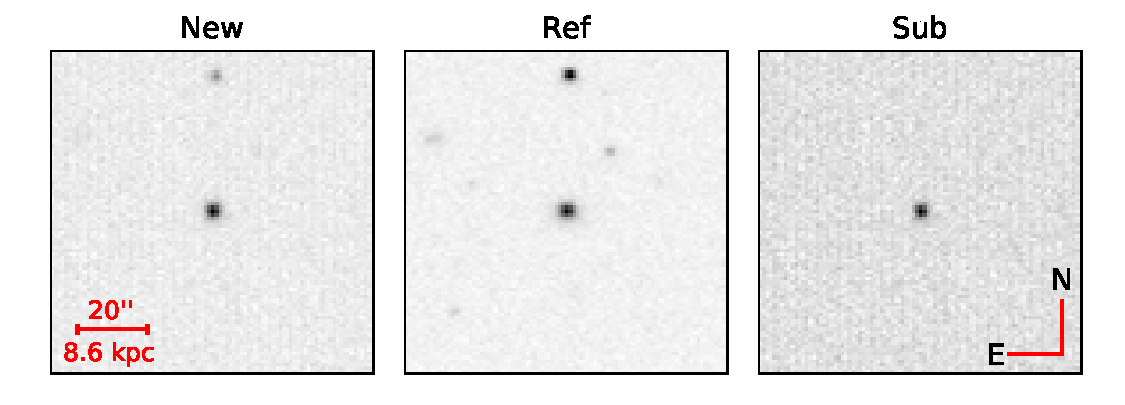
\includegraphics[width=\columnwidth]{figures/detection.pdf}
    \caption{ZTF $g$ band images centered on AT2019dge on Apr 10. From left to right are the new 
    image, the reference image, and the subtraction image. \ \label{fig:detection}}
\end{figure}
\begin{figure}
	\centering
	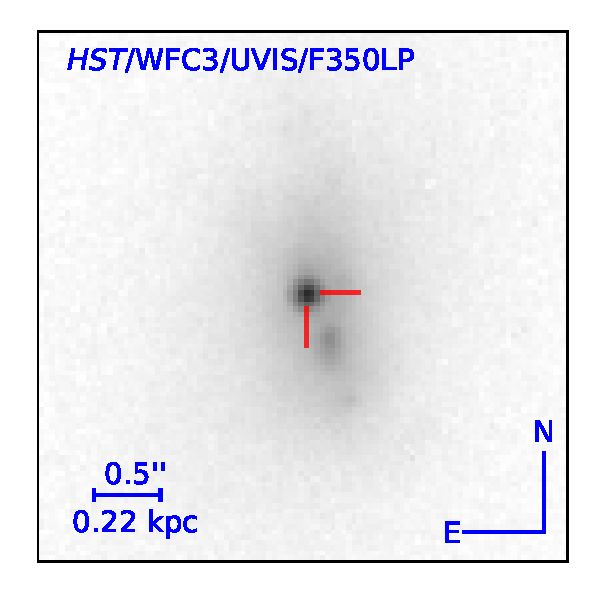
\includegraphics[width=0.6\columnwidth]{figures/offset.pdf}
	\caption{\textit{HST} image of the field on Apr 22 in the F350LP filter. The position of AT2019dge is 
	marked by the red crosshairs.
		%Images are combined using the prescription in \citet{Lupton2004}.
		\label{fig:offset}}
\end{figure}
\begin{figure*}[htbp!]
	\centering
	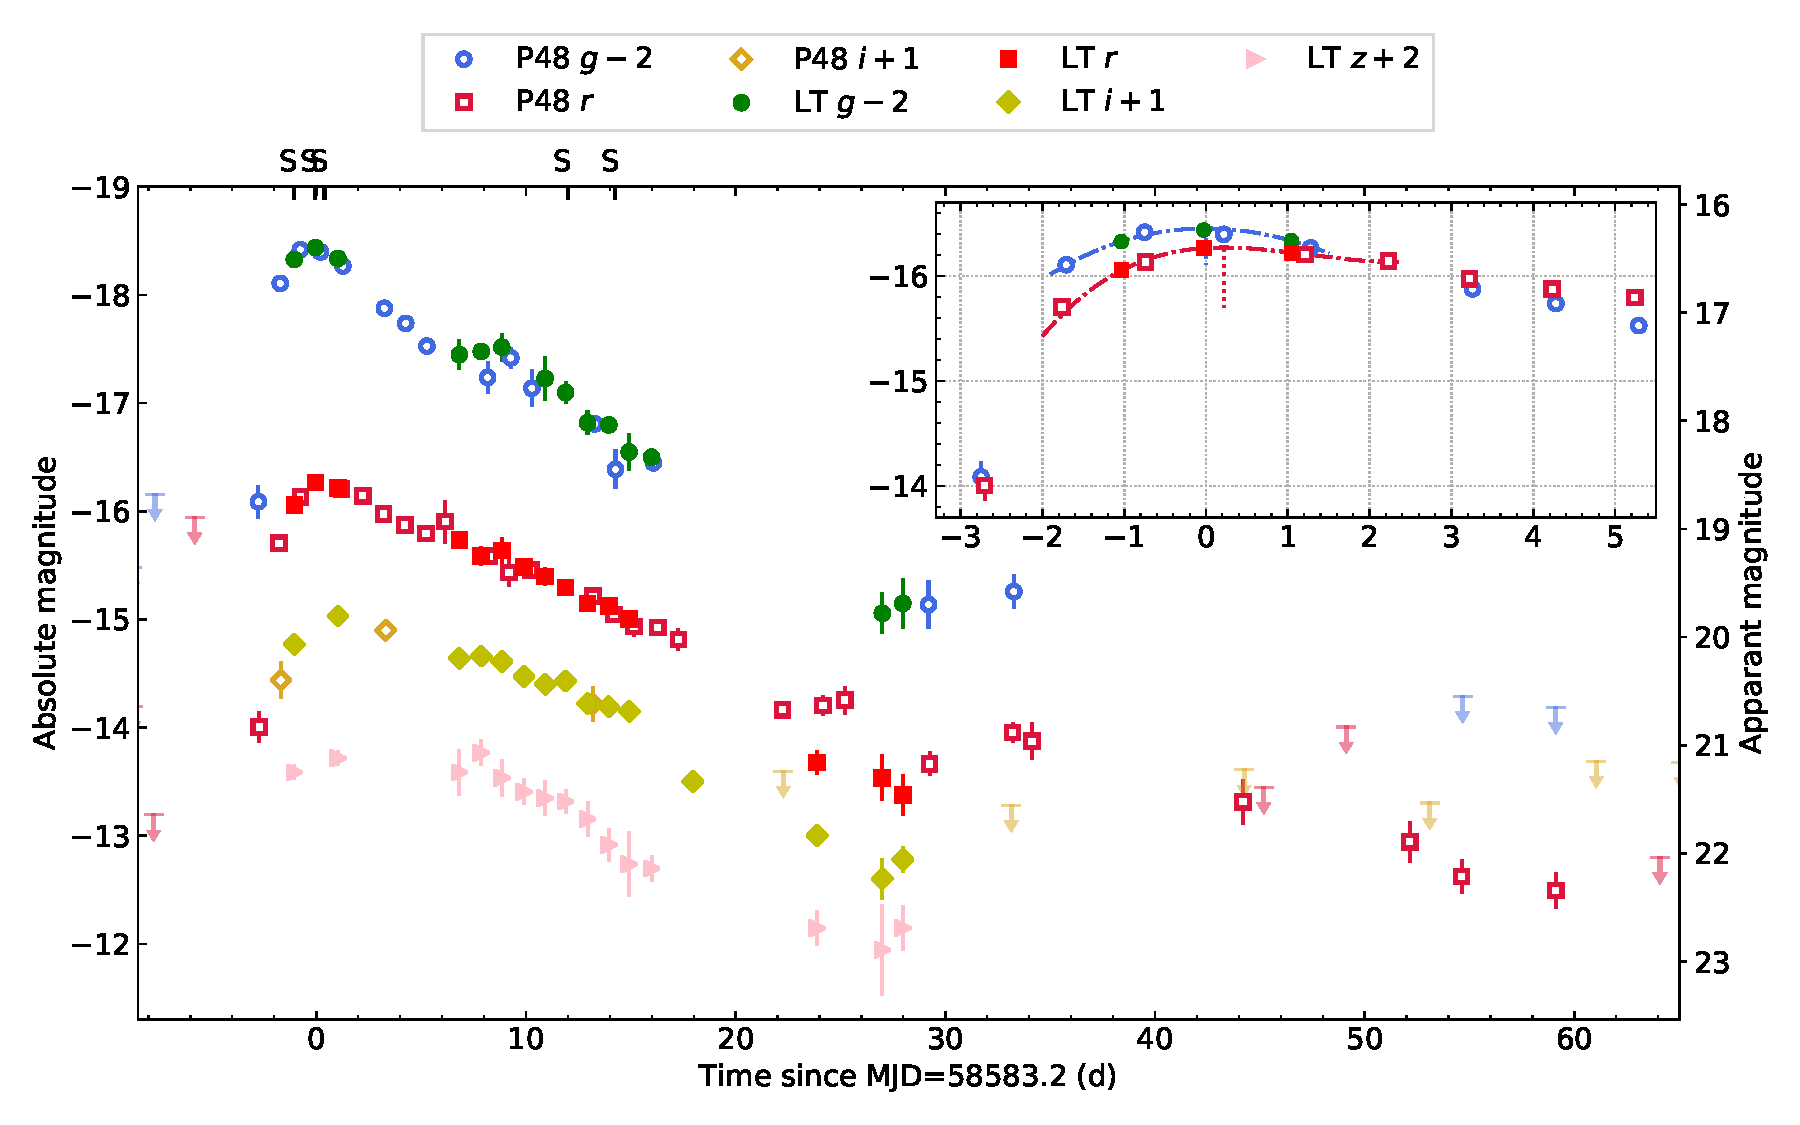
\includegraphics[width=\textwidth]{figures/lightcurve.pdf}
	\caption{Galactic extinction corrected light curve of AT2019dge. The inset shows 
		the light curve zoomed around the region of maximum light. Epochs of spectroscopy are marked 
		with the letter `S' along the upper axis.\label{fig:lightcurve}}
\end{figure*}
% In this section, I report values on Marshal
AT2019dge was first detected by ZTF, which runs on the Palomar Oschin Schmidt 48 inch (P48) 
telescope. The first real-time alert \citep{Patterson2019} was generated  on 2019 April 7 10:18:46 (JD 
$=2458580.9297$) for a $g$-band detection at $20.66\pm0.34$ mag and J2000 coordinates $\alpha 
= 17^{\mathrm{h}}36^{\mathrm{m}}46.75^{\mathrm{s}}$, $\delta = 
+50^{\mathrm{d}}32^{\mathrm{m}}52.2^{\mathrm{s}}$.
%$\alpha = 17^{\mathrm{h}}36^{\mathrm{m}}46.76^{\mathrm{s}}$, $\delta = 
%+50^{\mathrm{d}}32^{\mathrm{m}}52.5^{\mathrm{s}}$ (J2000) 
On April 8, a new alert was flagged by a science program filter on the 
GROWTH Marshal \citep{Kasliwal2019} that is designed to look for fast evolving transients. 
Figure~\ref{fig:detection} shows the ZTF detection image on April 10. AT2019dge resildes in a compact 
galaxy SDSS J173646.73+503252.3 at the redshift of $z=0.0213$ (See Appendix 
\ref{subsec:appspec_data}). 

\subsection{HST Observation}
HST observations are obtained as part of our  \textit{Hubble Space Telescope} ($HST$) ``Rolling 
Snapshots'' program (GO-15675, \citealt{Fruchter2018}). This new observational approach requires the 
PI to update a list of objects of interest each week before the schedule is build, giving the 
scheduler flexibility to choose a possible source of snapshots. Under this program, we obtained a NUV 
spectrum using the WFC3 G280 grism, a short (60\,s) direct image of this field in the F300X filter to 
set the wavelength scale of the  spectrum, as well as a longer exposure (200\,s) in the F350LP filter. 
The image in the F350LP filter is shown in Figure~\ref{fig:offset}. It has very similar throughput to the 
zeroth order of the G280 grism. We convolved this image to match the slight blurring of the zeroth 
order G280 grism and then scaled and subtracted it, dramatically reducing host contamination from 
the zeroth order host image.

 Since AT2019dge is offset from the nucleus of the host in Figure~\ref{fig:offset}, the explosion can 
 not be a  tidal distruption event.
 
\subsection{Photometry}
\subsubsection{Optical Photometry}
We perform forced PSF photometry on ZTF difference images following the steps illustrated in 
\citet{Yao2019}. The sky region of AT2019dge is covered by two ZTF fields with fieldid 763 and 
1799. We exclude all data in field 1799 since the reference image was constructed using images 
obtained between May 25 2018 and July 12 2019 (see \citealt{Masci2019} fordetails of  reference image 
generation), which is after the explosion of the transient. Although the ZTF name of this object 
(ZTF18abfcmjw) may indicate that the transient was discovered in 2018, this is due to an alert 
generated on July 7 2018 from a candidate detection in negative subtraction (reference minus science) 
in field 763. We note that the seeing at that night was 4.2 arcsec, larger than 99\% of Palomar nights. 
The irregular-shaped PSF might caused over-subtraction around the galaxy nucleus in the difference 
imaging process.

Since field 763 was included in both the northern sky survey with two epochs (one 
$g\, +$ one $r$) per three nights and the extragalactic high-cadence survey with six epochs (three 
$g\,+$ three $r$) per night (see \citealt{Bellm2019a} for the ZTF experiments design), this 
transient are visited muliple times every night. Therefore, single-night flux measurements in the same 
filter are binned (by taking the inverse variance-weighted average). This gives a pre-explosion 
$r$-band limit of 18.95 mag (5$\sigma$ limit computed at the expected position of the transient) on 
April 4 10:36:34. Five-$\sigma$ detections are converted to magnitude for further analysis.

Following the discovery of AT2019dge, we obtained follow-up photometry in $griz$ with the optical 
imager (IO:O) on the Liverpool Telescope (LT; \citealt{Steele2004}). Digital image subtraction and 
photometry for LT imaging was performed using the Fremling Automated Pipeline (\texttt{FPipe}; 
\citealt{Fremling2016}). \texttt{Fpipe} performs calibration and host subtraction against Sloan Digital 
Sky Survey reference images and catalogs (SDSS, \citealt{Alam2015}).

LT and P48 photometry are shown in Figure~\ref{fig:lightcurve}. Absolute magnitude is determined by 
correcting for the distance modulus 
and Galactic extinction $E(B-V)=0.022$ estimated by \citet{Schlafly2011}, which builds upon 
\citet{Schlegel1998}. We assume $R_V=3.1$, and adopt reddening law from \citet{Cardelli1989}. We do 
not correct for host-galaxy contamination given the absence of \ion{Na}{I} D absorption in all spectra 
at the host redshift. 

We also performed forced photometry on archival PTF/iPTF difference images spanning May 07 2009 to 
June 13 2016\footnote{We followed the procedure described in 
	\url{http://web.ipac.caltech.edu/staff/fmasci/home/miscscience/forcedphot.pdf}}. No historical 
detection was found. 
\subsubsection{Swift Photometry}
Space-based observations with the \textit{Neil Gehrels Swift Observatory} (\textit{Swift}; 
\citealt{Gehrels2004}) was triggered on April 9 and April 10. Ultraviolet/Optical Telescope (UVOT; 
\citealt{Roming2005}) data were obtained in the $UVW1$, $UVM2$, $UVW2$, $U$, $B$, and $V$ 
filters. 

UVOT data are reduced using HEAsoft (v6.17) with a $3^{\prime\prime}$ circular aperture. To remove 
host-galaxy contribution at the location of the SN, we obtained a final epoch in all broad-band filters 
on June 23 2019 and measured the photometry with the same aperture used for the transient. We 
present a table of our optical and UV photometry in Section \ref{subsec:appphot_data}.

We note that no point sources were detected in the XRT event files with $\rm{SNR}>3$.
The 3$\sigma$ limits in count\,s$^{-1}$ in the April 9, April 10, and June 23 observations are $7.8\times 
10^{-3}$,  $5.8\times 10^{-3}$, and $6.1\times 10^{-3}$, respectively.

\subsubsection{Radio Follow-up}
Shortly after the discovery of AT2019dge, we initiated radio follow-up in order to constrain the 
presence of a radio counterpart, as potentially expected in some rapidly-rising transients with 
circumstellar interaction \citep{HoPhinney2019}. We observed at high frequency radio bands using the 
Submillimeter Array (SMA, \citealt{Ho2004}) on UT 2019 Apr 09 between 15:49:17 and 19:51:26 UTC 
under its target-of-opportunity program. The 
project ID is 2018B-S047 (PI: Anna Ho). We did not detect AT2019dge in the resulting image, while we 
can place 3$\sigma$ upper limits to the flux density of 2.25\,mJy at 230\,GHz and 8.4\,mJy at 
345\,GHz. 
%The actual rms are 0.75 mJy for the 230 GHz image and 2.8 mJy for the 345 GHz image.

\subsection{Spectroscopy}

We obtained eight optical spectroscopic follow-up of AT2019dge from $-1.1$\,d to $+314.4$\,d relative 
to $g$-band peak using the Rapid Acquisition of Transients (SPRAT; \citealt{Piascik2014}) on the 
Liverpool Telescope (LT), the Double Spectrograph (DBSP) on the 200-inch Hale telescope 
\citep{Oke1982}, and the Low Resolution Imaging Spectrograph (LRIS) on the Keck-I telescope 
\citep{Oke1995}. To extract the LT spectra, we use the automated SPRAT reduction pipeline, which is a 
modification of the pipeline for FrodoSpec \citep{Barnsley2012}. The DBSP spectrum was reduced using 
a \texttt{PyRAF}-based reduction pipeline \citep{Bellm2016}. LRIS 
spectra were reduced and extracted using \texttt{Lpipe} \citep{Perley2019lpipe}. 

A log of our spectroscopic observations is presented in Appendix \ref{subsec:appspec_data}. We 
present our sequence of spectra in Figure~\ref{fig:spectra_early}, Figure~\ref{fig:spectra} and 
Figure~\ref{fig:spectra_late}.

\section{Properties of the Explosion \\and Its Host Galaxy}
\subsection{Light Curve Properties}\label{subsec:lc_properties}

\subsubsection{Peak Luminosity, Rise and Decline Timescale}
To estimate the epoch of maximum light, we interpolated the $g$- and $r$-band photometry with 
three-order polynomial functions, as is shown in the inset of Figure~\ref{fig:lightcurve}. The time range 
used in the fit is from ${\rm MJD}=58581.2$ to $58585.2$. AT2019dge was found to peak 
at $M_{g\rm , peak}=-16.45\pm0.04$ mag on ${\rm MJD}=58583.19$, and $M_{r \rm ,peak } 
=-16.27\pm0.02$ mag on ${\rm MJD}=58583.39$. Hereafter we use phase ($\Delta t$) to denote time
with respect to the $g$-band maximum light epoch, ${\rm MJD}=58583.2$.

The $g$- and $r$-band peak luminosity of AT2019dge ($\approx -16.3$\,mag) is around the lower limit 
of stripped envelope SNe, and similar to those of the Ca-rich gap transients, which occupy the 
luminosity `gap' between novae and SNe (peak absolute magnitude $M_R \approx 
-15.5$ to $-16.5$\,mag).

\begin{figure}[htbp!]
	\centering
	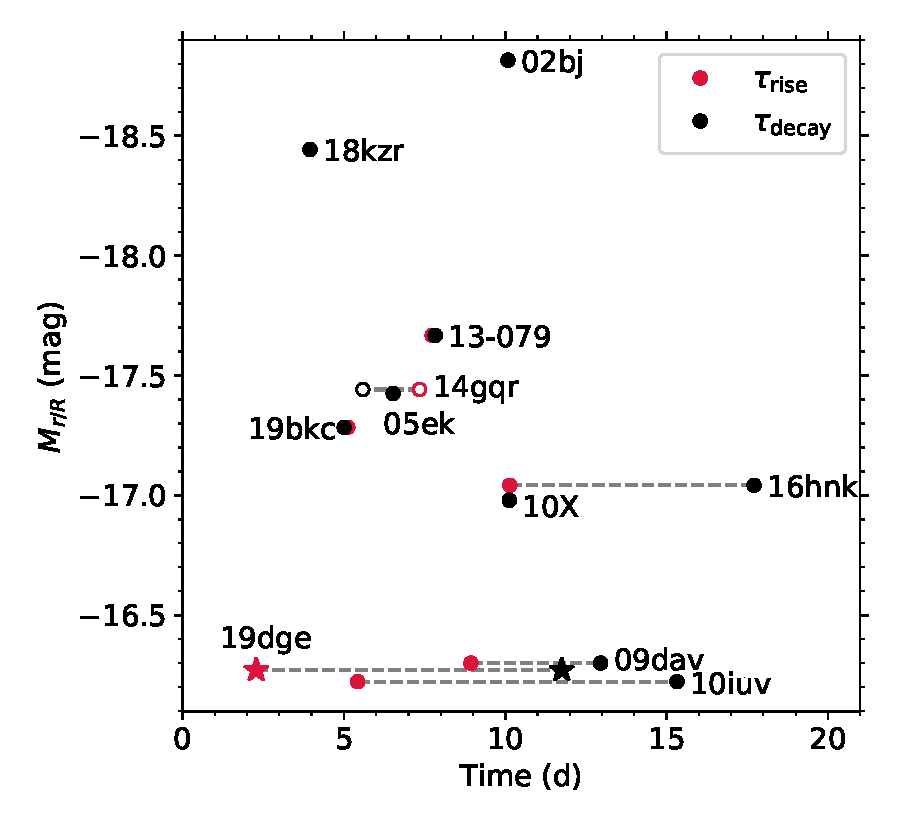
\includegraphics[width=\columnwidth]{figures/compare_mag.pdf}
	\caption{Comparison of the photometric evolution timescales ($t_{\rm rise}$ and $t_{\rm  
			decay}$) and peak absolute magnitude of AT2019dge to other H-deficient fast-evolving SNe, 
		including
		SN2002bj \citep{Poznanski2010},
		SN2005ek \citep{Drout2013},  
		PTF09dav \citep{Sullivan2011},
		SN2010X \citep{Kasliwal2010},
		PTF10iuv \citep{Kasliwal2012},
		iPTF14gqr \citep{De2018},
		KSN2015K \citep{Rest2018},
		 iPTF16asu	\citep{Whitesides2017}, 
		 iPTF16hgs \citep{DeKC2018},
		SN2018gep \citep{Ho2019},
		SN2018kzr \citep{McBrien2019}, 
		and SN2019bkc \citep{Chen2020}. See the text for details.
		\label{fig:compare_mag}}
\end{figure}


To characterize the rise and decline timescales of AT2019dge, we calculate rise time ($t_{\rm rise}$) 
defined by how long it takes the $r$-band light curve to rise from 0.75\,mag below peak to peak, 
and decline time ($t_{\rm decay}$) determined by how long it takes to decline from peak by 0.75\,mag 
(corresponding to half of maximum flux). In Figure \ref{fig:compare_mag} we compare the rise time, 
decay time, and peak absolute magnitude between AT2019dge and other fast-evolving 
hydrogen-deficient transients from the literature. 

In Figure \ref{fig:compare_mag}, peak magnitudes is given in $r$-band, except for KSN2015K where we 
only have observations in the \textit{Kepler} white filter, and iPTF16asu where the rise was only 
caught in $g$-band (but in rest-frame $r$-band since this is a high-redshift event). We only correct 
for Galactic extinction to compute $M_{r\rm , peak}$ (assming no host extinction). Note that 
iPTF14gqr and iPTF16hgs are two SNe exhibiting double peaked light curves. Since rising of their first 
peaks were not captured, an upper limit of $t_{\rm rise}$ is calculated by taking the time difference 
between the first $r$-band detection and the latest pre-discovery non-detection. Absolute magnitude 
of the first $r$-band detection is considered to be a fainter limit of $M_{r\rm , peak}$ (plotted in the 
upper panel). In the lower panel, since observation of iPTF14gqr does not extend to 0.75\,mag below 
its second peak, we present a lower limit of its $t_{\rm decay}$.

It is clear from the upper panel that AT2019dge rose faster than normal Ca-rich events such as 
PTF09dav and PTF10iuv. The rise time of $\approx 2$\,d is similar to some fast evolving luminous 
transients (FELTs) such as KSN2015K, iPTF16asu, and SN2018gep, but AT2019dge is substantially 
fainter than FELTs. In the subluminous regime, iPTF14gqr and likely iPTF16hgs have $t_{\rm rise}$ 
comparable to AT2019dge. Their first peaks have been postulated to be caused by the diffusion of 
shock-deposited energy out of an envelope around the progenitor star \citep{De2018, DeKC2018}.
 
The bottom panel of Figure \ref{fig:compare_mag} shows that $t_{\rm decay}$ of AT2019dge is 
longer than the most rapidly-fading SNe Ibc, such as SN2005ek, SN2018kzr, 
and SN2019bkc. Its decay timescale is more similar to SN2002bj, SN2010X, the population of Ca-rich 
transients (PTF09dav, PTF10iuv, iPTF16hgs) and likely iPTF14gqr. It has been suggested that the latter 
group of events have radioactivity powered main peak with low mass of nickel ($M_{\rm Ni} \lesssim 0.1 
M_\odot$).

\subsubsection{Bolometric Evolution}
\begin{figure}[!htbp] 
	\centering
	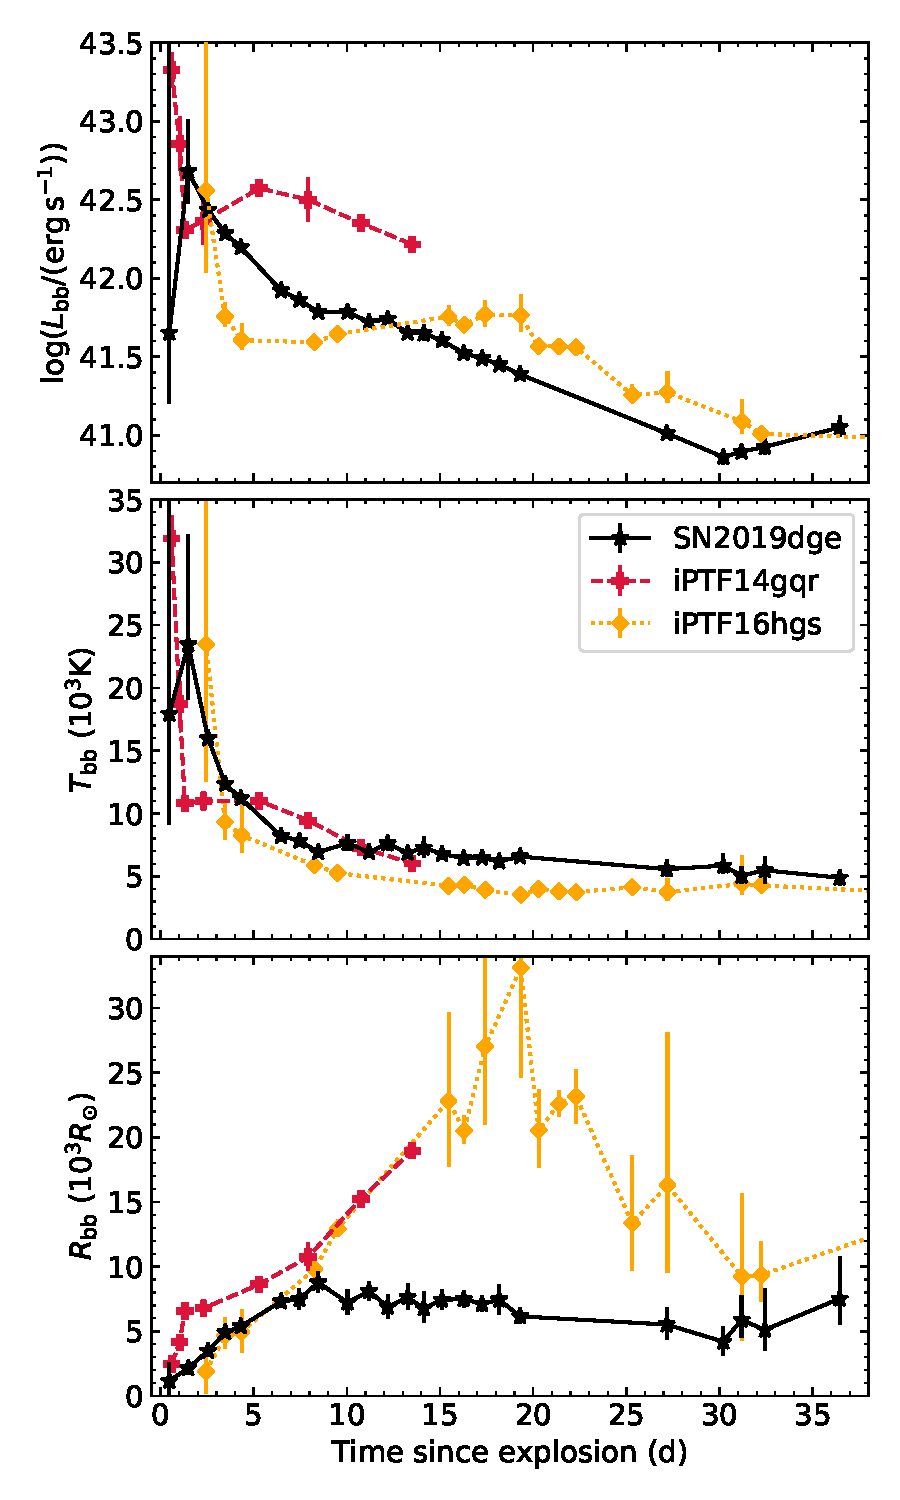
\includegraphics[width=\columnwidth]{figures/Tbb_Rbb.pdf}
	\caption{Evolution of blackbody properties (lumionosity, temperature, radius) over time of 
		AT2019dge compared to iPTF14gqr and iPTF16hgs. We adopt blackbody parameters of iPTF14gqr 
		provided by \citet{De2018}, and use the same method as applied in AT2019dge to derive 
		parameters of iPTF16hgs. At epochs where data in more than two filters are available, estimated 
		values are plotted in solid dots, whereas estimates from only two filters are shown in empty 
		circles.}
	\label{fig:Tbb_Rbb_Lbb}
\end{figure}
\begin{figure*}[htbp!]
	\centering
	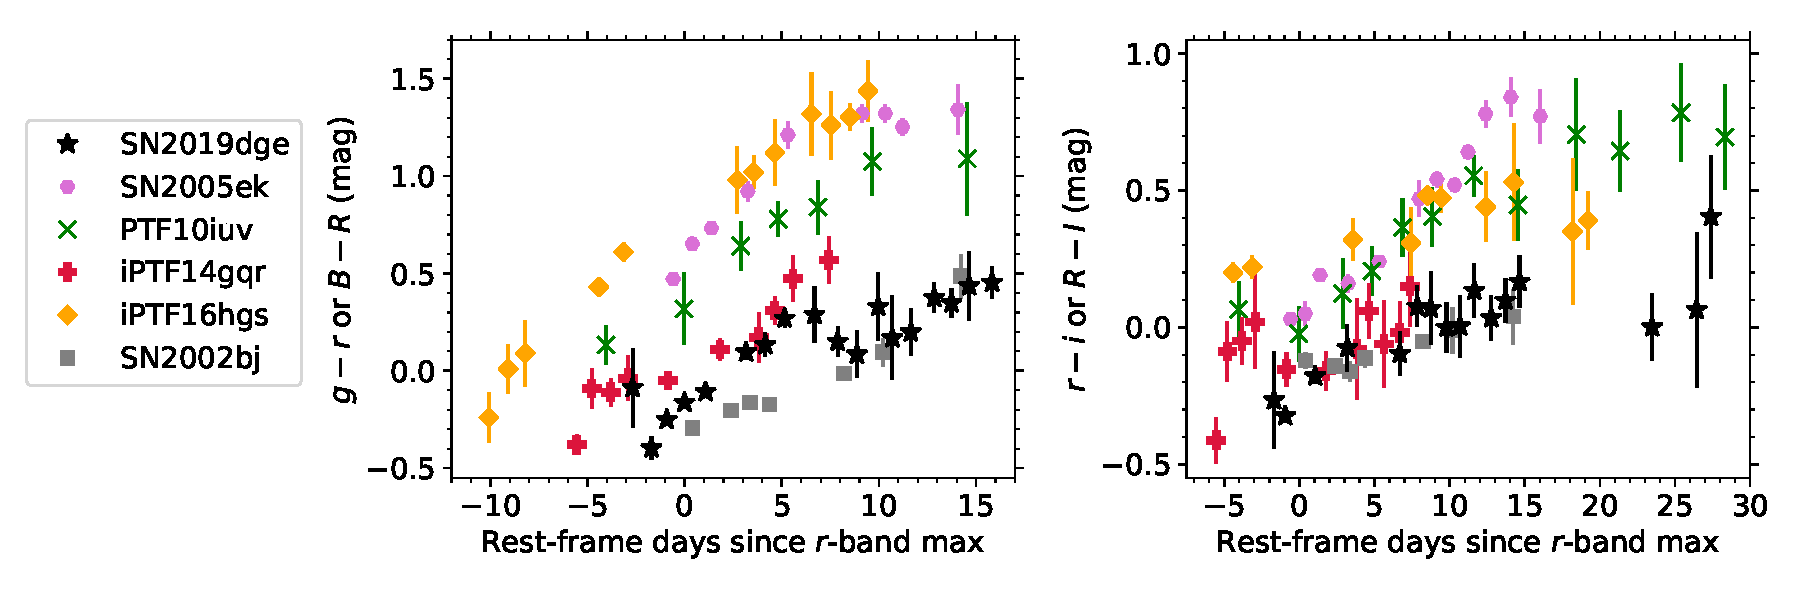
\includegraphics[width=\textwidth]{figures/compare_color.pdf}
	\caption{Comparison of the color evolution of AT2019dge with a subset of fast SNe shown in 
		Figure~\ref{fig:compare_mag}. All colors have been corrected for Galactic extincton. Due to 
		absence of photometry in identical filters, we compare colors in corresponding filter pairs of 
		$B$/$g$, $R$/$r$ and $I$/$i$.  \label{fig:compare_color}}
\end{figure*}

We constructed the bolometric light curve evolution by fitting a blackbody function to the spectral 
energy distribution (SED). At eighteen epochs where at least detections in three flters are available, we 
utilized the Monte Carlo Markov Chain (MCMC) simulations with \texttt{emcee} 
\citep{Foreman-Mackey2013} and adopted wide and flat prior for the blackbody radius and 
temperature ($0<T_{\rm bb}<10^6$\,K, $0<R_{\rm bb}<10^6\,R_\odot$). Uncertainties are estimated 
using the difference between the 84th and the 16th percentiles of posterior probability distributions. At 
five epochs that we only have photometric observations in two filters, we fit for $T_{\rm bb}$ and 
$R_{\rm bb}$ with no estimates on the parameter uncetainties. The SED fits are shown in 
Appendix \ref{subsec:appphot_data}. 

In Figure~\ref{fig:Tbb_Rbb_Lbb}, we plot the physical evolution of AT2019dge with a comparison to 
iPTF14gqr and iPTF16hgs. We adopt the explosion epoch of iPTF14gqr, iPTF16hgs, and AT2019dge 
estimated by \citet{De2018}, \citet{DeKC2018}, and Section \ref{subsec:fastrise} of this paper, 
respectively. The bolometric luminosity of AT2019dge reaches $\sim 5\times 10^{42}\,{\rm erg\, s^{-1}}$ 
at $\sim 1.5$\,d after the assumed explosion epoch. The subsequent decline displays an initial 
fast drop of $0.36\,{\rm mag\,d^{-1}}$ at age 2--7\,d, and transitions to a slower drop of $0.11\,{\rm 
mag\,d^{-1}}$ at age 8--30\,d. Noe that data points of AT2019dge at age 0.5\,d are plotted in 
empty circles, indicating that no uncertainties can be obtained and their values should only be 
considered as rough estimates. 

The bolometric temperature of AT2019dge reaches as high as $\sim 2.3\times 10^4$\,K at age $1.5$\,d 
and rapidly falls afterwards. The maximum $T_{\rm bb}$ is much hotter than that observed in normal 
SNe Ibc (6000--10000\,K, \citealt{Taddia2018}). Its early evolution is less fast than iPTF14gqr, but 
similar to iPTF16hgs and several other stripped envelope SNe displaying double-peaked light curve 
(e.g., see Figure~2 of \citealt{Fremling2019}). Their first peaks have been modelled by cooling emission 
from an extended envelope around the progenitor after the core-collapse SN shock breaks out 
\citep{Modjaz2019}. After $\sim 8$\,d past explosion, $T_{\rm bb}$ flattens to $6000\pm1000$\,K, 
similar to the behavior of normal SNe Ibc at a much later phase ($\sim30$\,d after explosion, 
\citealt{Taddia2018}).

Assuming that the photospheric radius can be approximated by $R_{\rm bb}$ and linearly expands at 
early phase, we fit a linear function to the first few $R_{\rm bb}$ vs.~time measurements of AT2019dge 
(lower panel of Figure \ref{fig:Tbb_Rbb_Lbb}), which gives $\approx 8150\, {\rm km\,s^{-1}}$. The radius 
remains flat at $\sim 6.6\times 10^3\,R_\odot$ during age 8--30\,day, and even appears to slowly 
recede. The total integrated blackbody energy output during $ t = 0.5$--30\,d is $\sim 2\times 
10^{43}\,{\rm erg\,s^{-1}}$. 

\subsubsection{Color Evolution}
We compare the color curves of other fast transients to that of AT2019dge in 
Figure~\ref{fig:compare_color}, in corresponding pairs of $B$/$g-R$/$r$ and $R$/$r-I$/$i$ colors. For 
double-peaked events iPTF14gqr and iPTF16hgs, ``maximum'' time corresponds to epoch of maximum 
light in the second peak.

The early-time blue color of AT2019dge arises from the high-temperature peak. Among other events, 
SN2002bj, iPTF14gqr and iPTF16hgs exhibit earliest colors as blue as AT2019dge. Subsequently, 
AT2019dge displays a color starting out blue and turning redder with time, consistent with a cooling 
process. 

One uniqueness of AT2019dge is that at 6--9 days after maximum light, the $g-r$ color becomes bluer 
by $\approx 0.2$\,mag, while after that the color continues to redden. We notice that iPTF14gqr also 
exhibit this behavior --- around 4\,day before the second peak, its $g-r$ color stays flat before getting 
redder afterwards, while around 2\,day before the second peak, its $r-i$ color alsp turns bluer by 
$\approx 0.2$\,mag.

\begin{figure*}[htbp!]
	\centering
	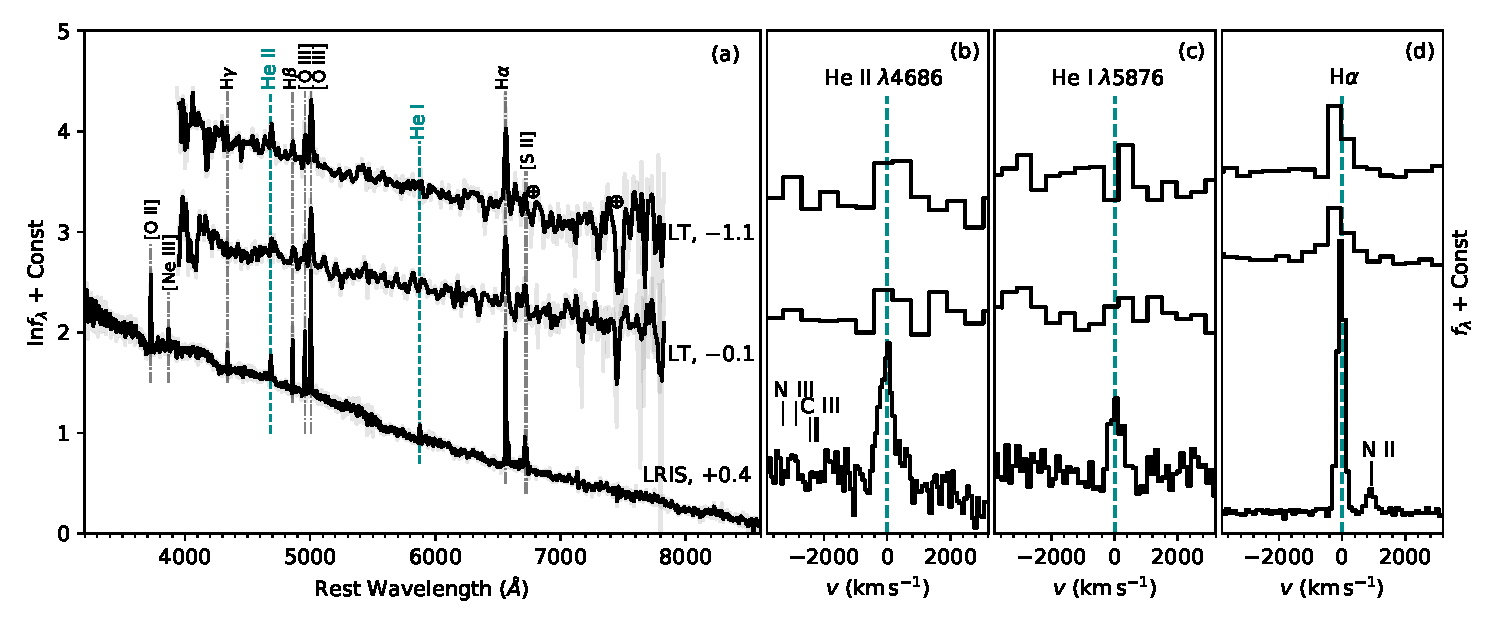
\includegraphics[width=\textwidth]{figures/spectra_early.pdf}
	\caption{Early-time spectra of AT2019dge.  In panel (a), the original spectra are	
		shown in translucent colors, with the overlying black lines showing the same spectra convolved 
		with an ${\rm FWHM} = 800\, {\rm km\, s^{-1}}$ (for LT)  or ${\rm FWHM} = 200\, {\rm km\, 
			s^{-1}}$ (for LRIS) Gaussian kernel. Prominent galaxy lines are marked by the 
		dash-dotted lines. In panel (b) (c) and (d), we show the observed spectra (not convolved with any 
		kernels) in velocity space around the \ion{He}{II} $\lambda 4686$, \ion{He}{I} $\lambda 5876$ and 
		H$\alpha$ emission lines.
		\label{fig:spectra_early}}
\end{figure*}

\begin{figure*}[htbp!]
	\centering
	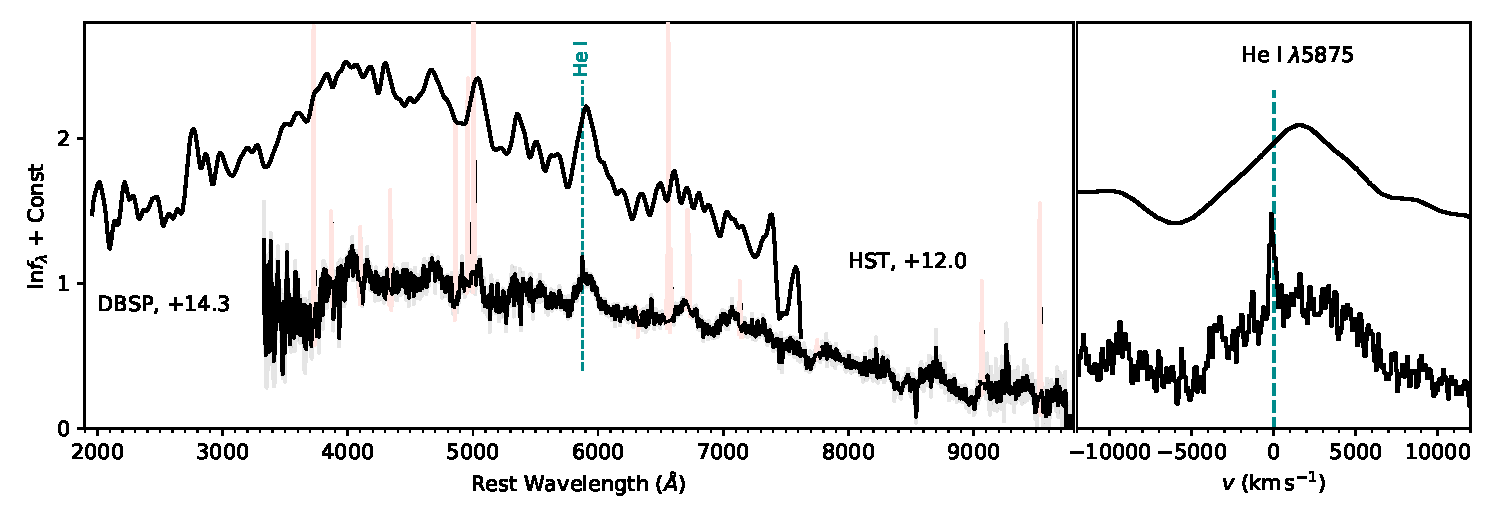
\includegraphics[width=\textwidth]{figures/spectra_phot.pdf}
	\caption{Photosperic phase spectra of AT2019dge. In panel (a), the original DBSP 
	spectrum is shown in translucent colors, with the overlying black lines showing the same spectrum 
	convolved with an ${\rm FWHM} = 200\, {\rm km\, s^{-1}}$ Gaussian kernel. We mask prominent 
	galaxy lines in the DBSP spectrum in light red. In pabel (b), we show the observed spectra (not 
	convolved with any kernels) in velocity space around \ion{He}{I} $\lambda 5876$ .
		\label{fig:spectra}}
\end{figure*}

\subsection{Spectroscopic Properties}\label{subsec:spec_properties}
The phases of the spectra indicated in this section are relative to $r$-band peak.
\subsubsection{Early Spectral Evolution} \label{subsubsec:spec_early}
The very early spectra at $-1.1$, $-0.1$, and $+0.4$\,d show a blue continuum and strong galaxy 
emision lines from the underlying \ion{H}{II} region (see Figure~\ref{fig:spectra_early}). In 
addition, these spectra also show prominent \ion{He}{I} $\lambda5875$ and high-ionization \ion{He}{II} 
$\lambda4686$ narrow emission lines. Using the line index definition given by \citet{Khazov2016}, we 
calculated the equivalent width of \ion{He}{II} to be $-7.56\pm 1.07$ 
$-2.66\pm 1.30$, and $-3.77\pm 0.16$ in the $-1.1$\,d, $-0.1$\,d, and $+0.4$\,d spectra. Full-width at 
half-maximum intensity (FWHM) velocities of the \ion{He}{II}, \ion{He}{I}, and H$\alpha$ emission lines 
are $\sim 550\,{\rm km\,s^{-1}}$, $\sim 570\,{\rm km\,s^{-1}}$, and $320\,{\rm km\,s^{-1}}$ (unresolved), 
respectively. Thus, we infer that the hydrogen emission is from the host galaxy, while the helium lines 
are from photoionized material in a region of immediate environment exterior to the SN.

Early-time low-velocity \ion{He}{II} $\lambda4686$ emission has been detected in nearly twenty
hydrogen-rich CCSNe and one hydrogen-poor SN iPTF14gqr. This feature often fades away within a 
few hours to a few days after the explosion \citep{Yaron2017}. The high ionization potential of this line 
requires high temperature or an ionizing flux, which might come from either shock breakout or CSM 
interaction \citep{GalYam2014, Smith2015}. Due to the rapid decrease in $T_{\rm bb}$ at the three 
epochs of our early-time spectra and the similarity between AT2019dge and iPTF14gqr, we favor shock 
cooling emission as the origion of recombination helium lines.

\subsubsection{Photosperic Phase Spectral Evolution}

\begin{figure}[htbp!]
	\centering
	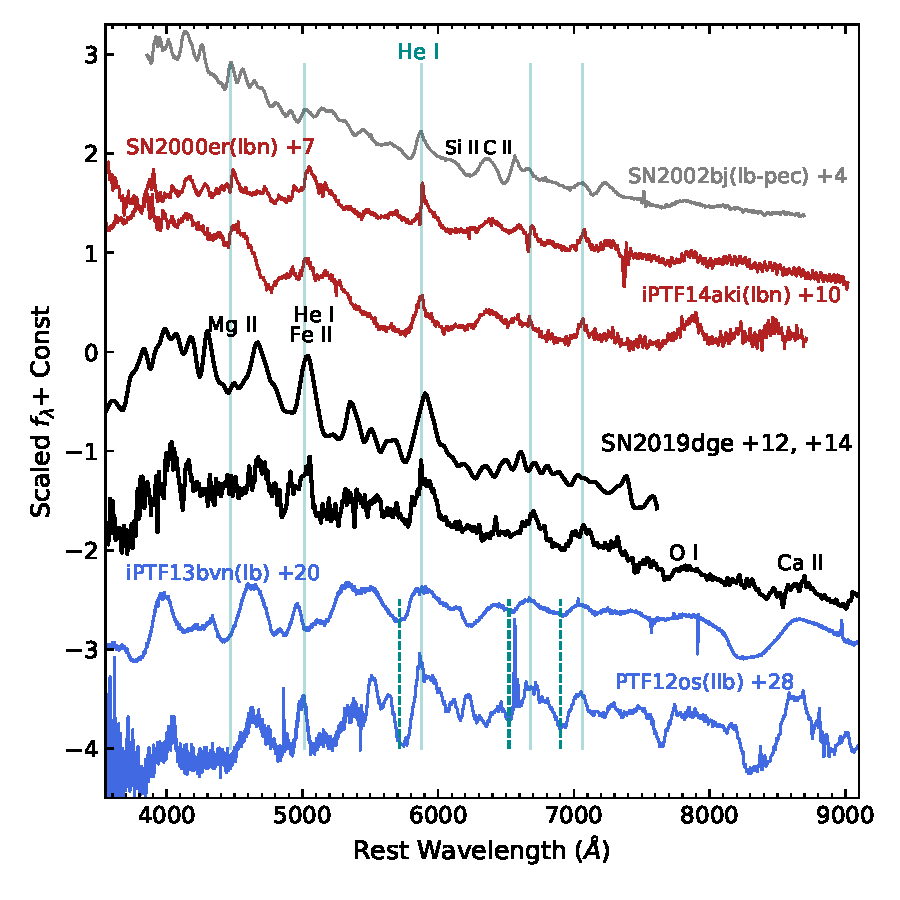
\includegraphics[width=\columnwidth]{figures/hst_opt.pdf}
	\caption{Photosperic phase spectra of AT2019dge compared with 
		other SNe, including SN2000er \citep{Pastorello2008}, SN2002bj \citep{Poznanski2010}, iPTF14aki 
		\citep{Hosseinzadeh2017}, PTF12os and iPTF13bvn \citep{Fremling2016}. \ion{He}{I} transitions at 
		rest wavelength are marked by the vertical cyan lines (though note that not all of these lines are 
		visible in all spectra shown here).
		\label{fig:hst_opt}}
\end{figure}

Broad transient features show up in the $+12.0$ and $+14.3$\,d spectra (Figure~\ref{fig:spectra}). The 
HST spectrum contains little host-galaxy contamination 
due to its high angular resolution. Prominent galaxy emission lines in the DBSP 
spectrum are identified and plotted in light red to emphasize transient features. The existence of 
P-Cygni \ion{He}{I} $\lambda5876$ profile and non-existence of hydrogen is reminiscent of Type Ib SN. 
We measure the velocity of the \ion{He}{I} $\lambda5876$ line by fitting a parabola to the absorption 
minimum. The resulting fits give velocities of $\approx 6000\, {\rm km\,s^{-1}}$ and $ 5900\, {\rm 
km\,s^{-1}}$ for the $+12.0$\,d and $+14.3$\,d spectra, respectively. This is lower than velocities of 
normal SNe Ib measured from the \ion{He}{I} $\lambda5876$ absorption minimum ($\sim 10^4\, \rm km\, 
s^{-1}$, \citealt{Liu2016}), but higher than that in Type Ibn SNe ($\sim 3000\, \rm km\, s^{-1}$, 
\citealt{Hosseinzadeh2017}).

\begin{figure}[htbp!]
	\centering
	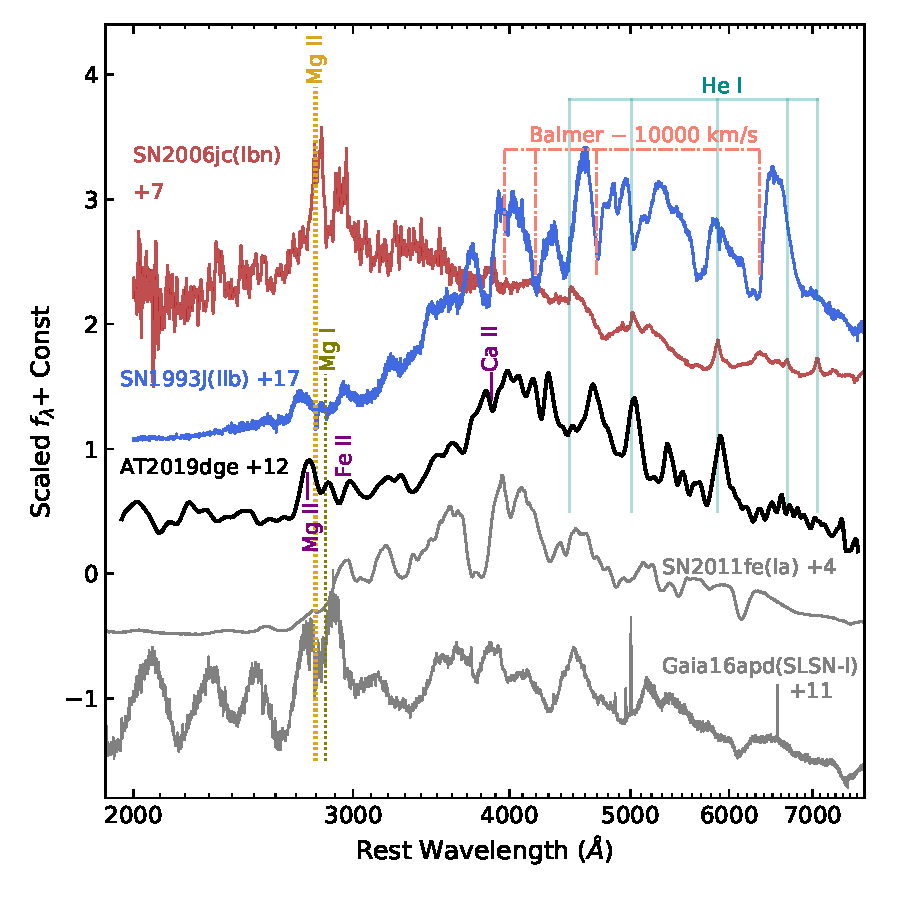
\includegraphics[width=\columnwidth]{figures/hst_all.pdf}
	\caption{HST spectrum of AT2019dge compared with other SNe, including SN2006jc 
		\citep{Bufano2009}, SN1993J \citep{Jeffery1994}, SN2011fe \citep{Mazzali2014}, and Gaia16apd 
		\citep{Yan2017}.
		\label{fig:hst}}
\end{figure}

In Figure~\ref{fig:hst_opt}, we compare the photosperic phase optical spectra of 
AT2019dge with other helium-rich events. Note that the DBSP specrum has host emission lines 
masked. AT2019dge is different from normal helium-rich stripped envelope SNe Ib/IIb or SNe Ibn in the 
sense that its P-Cygni absoprtion minimum in the \ion{He}{I} $\lambda5876$ line is much weaker. The 
feature at $\sim5000{\rm \AA}$ is often attributed to \ion{He}{I} $\lambda 5016$ and \ion{Fe}{II} triplet 
$\lambda\lambda\lambda4924$, 5018, and 5169 \citep{Liu2016}. The shape of this feature in 
AT2019dge is similar to normal SNe Ib/IIb at much later phase ($\sim 20$\,d post maximum), indicating 
that the spectral evolution of AT2019dge is faster. The complex absorption 
profile at $\sim4500{\rm \AA}$ has been identified as a blend of \ion{Fe}{II}, \ion{Mg}{II} $\lambda 4481$ 
and \ion{He}{I} $\lambda 4472$ \citep{Hamuy2002}. In the DBSP spectrum, we detected \ion{O}{I} 
$\lambda 7774$ and broad \ion{Ca}{II} at $\sim8500{\rm \AA}$ (due to the triplet at 8498, 8542, and 
8662\AA) with clear P-Cgyni profiles; Both are major features of stripped envelope SNe. 

In Figure~\ref{fig:hst}, we compare the HST NUV spectrum with other types of SNe. 
The UV part of AT2019dge is much weaker than a blackbody extrapolation of the optical spectra would 
predict. This has also been seen in normal thermonuclear and CCSNe, and interpreted as strong 
metal-line blanketing caused by iron-peak elements, particularly \ion{Fe}{II} and \ion{Co}{II} 
\citep{Gal-Yam2008}. AT2019dge bears a close resembance to SN1993J between 2000 and 4000\AA. 
In Figure~\ref{fig:hst} we also marked rest wavelength of \ion{Mg}{I} $\lambda2852$ and \ion{Mg}{II} 
$\lambda \lambda 2796$, 2803. The emission features at $\sim2760{\rm \AA}$ in AT2019dge and 
Gaia16apd are similar to the bump at $\sim2730{\rm \AA}$ in SN1993J, which was found to be a NLTE 
\ion{Mg}{II} emission line \citep{Jeffery1994}. This resonance line is blueshifted from its rest wavelength 
since the ejecta are very optically thick, and has been interpreted as interaction of the SN ejecta and a
circumstellar shell. Such an UV emitting shell may consist of gas originally ejected by the 
stellar progenitor as a stellar wind or during an episodic mass ejection. 

\subsubsection{Late-time  Spectral Evolution}
\begin{figure*}[htbp!]
	%
	\centering
	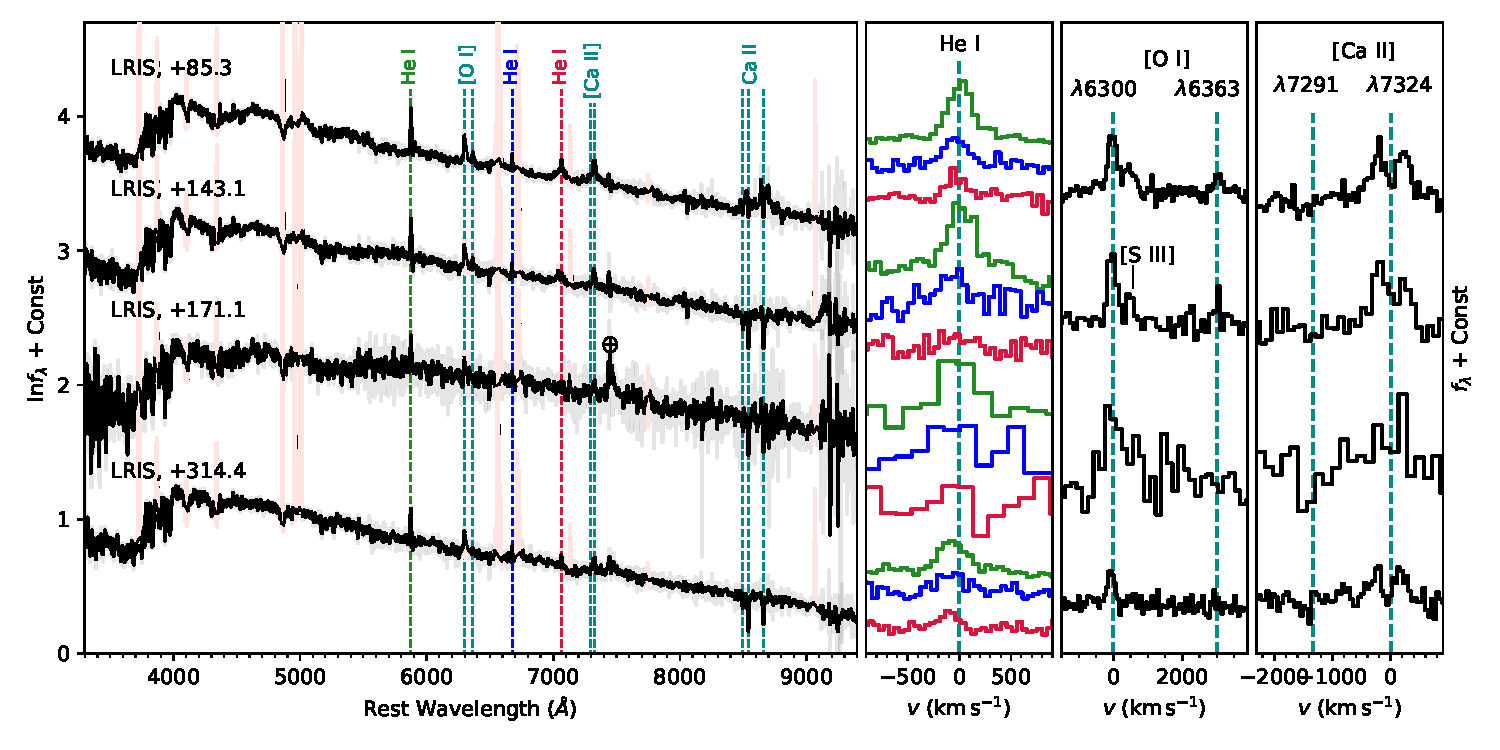
\includegraphics[width=\textwidth]{figures/spectra_late.pdf}
	\caption{Late-time spectra of AT2019dge. In panel (a), the original spectra are	
		shown in translucent colors, with the overlying black 
		lines showing the same spectra convolved with ${\rm FWHM} = 200\, {\rm km\, 
			s^{-1}}$ Gaussian kernels. We mask prominent galaxy lines in light red. Possible SN features are 
			marked by the dashed lines. In panel (b) (c) and (d), 
			 the spectra at phase $+85.3$\,d, $+143.1$\,d, $+171.1$\,d, and $+314.4$\,d, are 
			 binned by 1, 2, 3, and 1 pixel(s), respectively. The binning factors are chosen based on the 
			 different signal-to-noise ratio (SNR) in these spectra (see exposure times in 
			 Table~\ref{tab:spec}). Note that in panel (b), we plot evolution of \ion{He}{I} $\lambda 5876$, 
			 $\lambda 6678$, and $\lambda 7065$ emissions in green, blue, and crimson, respectively.
		\label{fig:spectra_late}}
\end{figure*}

\begin{figure*}
		\centering
	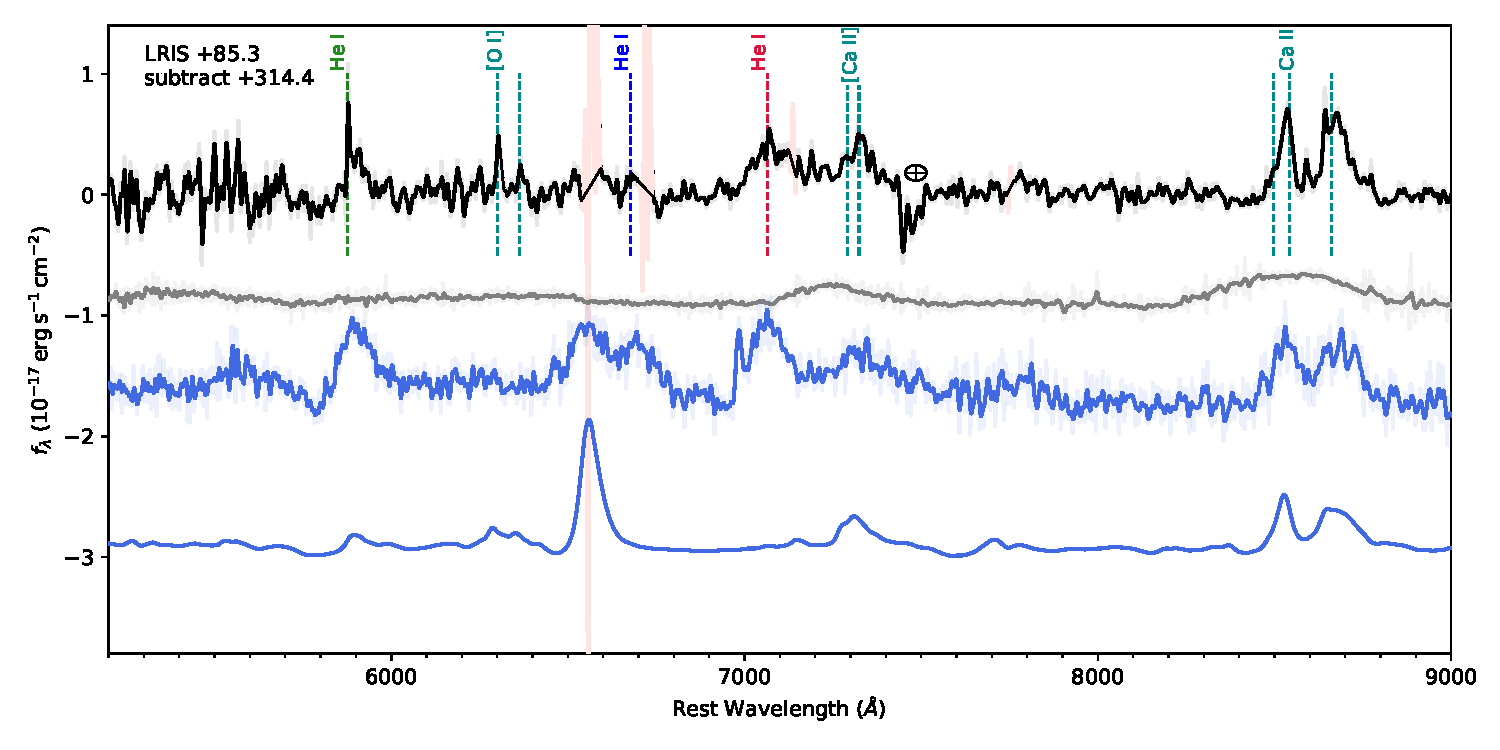
\includegraphics[width=\textwidth]{figures/spec_host_subtracted.pdf}
		\caption{Subtracted nebular spectrum of AT2019dge compared with Type Ibn SNe SN2006jc 
		\citep{Shivvers2019}, 
		SN2011hw \citep{Pastorello2015}, and SN2015G \citep{Shivvers2017}.
		\label{fig:spec_subtract}}
\end{figure*}
Panel (a) of Figure~\ref{fig:spectra_late} shows late time spectra of AT2019dge obtained at $+85.3$, 
$+143.1$, $+171.1$, and $+314.4$\,d.  The general shape of the spectra is determined by the host 
galaxy, while possible SN features are marked by the dashed lines. The right panels (b), (c), and (d) 
highlight emission lines at wavelengths of \ion{He}{I}, [\ion{O}{I}], and [\ion{Ca}{II}]. FWHM velosities 
of the narrow emissions are not well resolved $\sim 300\,{\rm km\,s^{-1}}$. 
The intensities decrease by a factor of approximately two from $+85.3$\,d to $+314.4$\,d. In panel (c), 
the [\ion{O}{I}] $\lambda \lambda 6300, 6363$ feature consists of two narrow emission 
peaks. This doublet transitions share the same upper level ($\rm ^{3}P_{1,2}$--$\rm ^{1}D_2$). The 
observed intensity ratio $R \equiv F(6300/6364) \sim 3.1$ agrees with the nebular condition, as one 
would expect in the optically thin regime. In panel (d), we mark position of the [\ion{Ca}{II}] 
$\lambda \lambda 7291$, 7324 doublet in dashed lines, but only the $\lambda 
7324$ line is clearly detected. It presents a double-peaked profile with a peak separation of $\sim 
400\,{\rm km\,s^{-1}}$. 
%\todo{I don't know why the 7291 narrow line is not observed, and the origin of 
%the double-peaked narrow compoennts}

To further investigate SN features from the galaxy light dominated spectra, we use the $+314.4$\,d 
spectrum as a galaxy template and subtract it from the $+85.3$\,d spectrum. The resulting subtraction 
(Figure~\ref{fig:spec_subtract}) reveals intermediate-width (FWHM $\sim 
2000\,{\rm km\,s^{-1}}$) components of \ion{He}{I}, [\ion{Ca}{II}], and \ion{Ca}{II} IR triplet ($\lambda 
\lambda \lambda 8498$, 8542, 8662), and shares a resemblance to some 
Type Ibn SNe, such as SN2011hw \citep{Pastorello2015} and SN2015G \citep{Shivvers2017}. These 
intermediate-width features are too narrow to be explained by emission from
radioactivity-heated optically thin SN ejecta. Instead, they are probably emitted by a dense  CSM shell 
formed by radiative cooling of the  post-shock material, as was proposed to be the case in interacting 
Type IIn/Ibn SNe \citep{Chugai1994, Smith2017}. 

The temporal evolution in strength of the narrow ($< 300\,{\rm km\,s^{-1}}$) lines shows that the 
emissions are connected to the explosion and are not merely a background contamination of an 
underlying \ion{H}{II} region. Such narrow lines have been observed at late-time in old nearby CCSNe 
such as Type Ib Type SN1985F \citep{Filippenko1989}, Type IIn SN1986J \citep{Leibundgut1991} and 
Type IIb SN1993J \citep{Matheson2000}. They were suggested to arise from dense clumpy regions in 
the SNe ejecta or circumstellar gas.

pre-shock circumstellar medium
(CSM).

Matheson 2001 \citep{Matheson2001}

The narrow components are not from the ejecta but instead from slow pre-shock CSM

\subsection{Host Galaxy Properties}
\begin{figure}[htbp!]
	\centering
	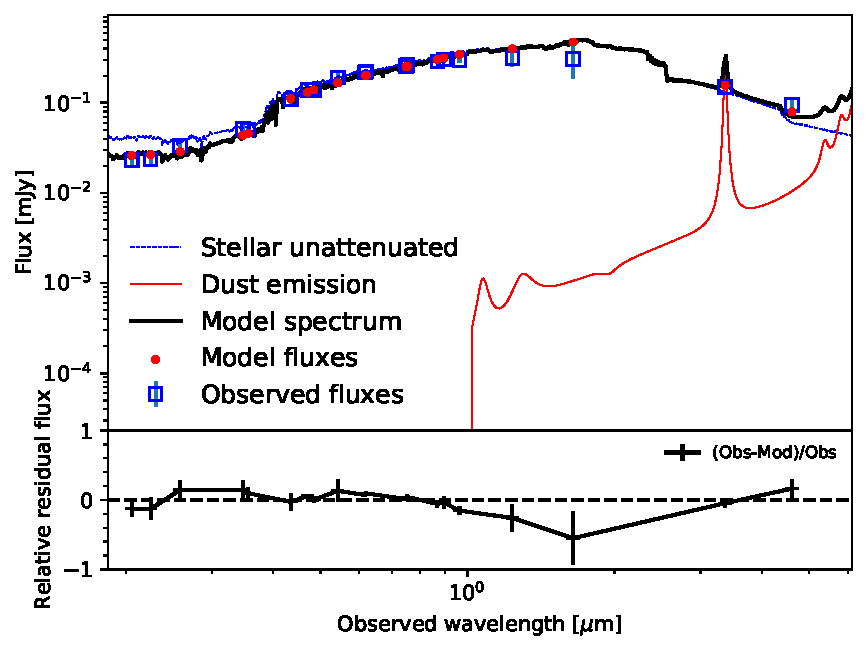
\includegraphics[width=\columnwidth]{figures/SDSSJ17+50_best_model.pdf}
	\caption{Spectral energy distribution of the host galaxy of AT2019dge. The observed photometric 
		data (with 1$\sigma$ error bars) are shown in blue open squares, and the model is shown in black 
		curve. The relative residual flux is shown in the bottom panel.
		\label{fig:SEDfit}}
\end{figure}

We measure the properties of the host galaxy using the spectrum obtained at phase $+314.4$\,d, 
assuming that the nebular line emissions are from the host galaxy. 

We infer a star-formation rate of $0.10 \pm 0.02 \, M_\odot\, {\rm yr^{-1}}$ from the H$\alpha$ 
emission line using the \citet{Kennicutt1998} relation converted to use a Chabrier initial mass function 
\citep{Chabrier2003, Madau2014}. 

We also compute the oxygen abundance using the strong-line metallicity indicator N2 
\citep{Pettini2004} with the updated calibration reported in \citet{Marino2013}. The oxygen abundance 
in the N2 scale is 8.23 $\pm$ 0.01 (stat) $\pm$ 0.05 (sys).

In Figure~\ref{fig:SEDfit} we shoulw the SED of xx, which was compiled from Swfit/UVOT, SDSS, PS1, 
2MASS,, and WISE catalogs. The measured host photometry is 
given in Table~\ref{tab:host_phot}.

\textcolor{red}{Zhihui:} 
We further determine the stellar mass ($M_{\star}$) of the host galaxy by SED modeling using 
\texttt{CIGALE} \citep{CIGALE19}. We adopt the stellar population synthesis models from \citet{BC03} 
with the Chabrier IMF \citep{Chabrier2003}, and assume a double declining  exponential star formation 
history (SFH). In addition, a dust component is added using the \citet{DL07} model to account for dust 
emission. Finally, the total SED model is attenuated by the Calzetti extinction curve \citep{Calzetti2000}.

The fitted SED is shown in Figure 7. The derived stellar mass is log $M_{\star}/M_{\odot}$ = 
$8.0 \pm 0.1$, and the SFR is $0.8 \pm0.1\, M_\odot\, {\rm yr^{-1}}$.

It is worth noting that while several 
previously reported events (SN\,2005ek, SN\,2010X, iPTF\,14gqr) and SN\,2018kzr were found in star 
forming host galaxies, SN\,2019bkc stands out as a hostless transient offset by tens of kpc from any 
likely host (see Table \ref{tab:compare}). 

Table \ref{tab:compare} shows a summary of our literature search.

\begin{deluxetable*}{lllll}[htbp!]
	\tablecaption{Summary of Subluminous Fast Transient. \label{tab:compare}}
	\tablehead{
		\colhead{Name}   
		& \colhead{Redshift} 
		& \colhead{Host} 
		& \colhead{Offset (kpc)}   
		& \colhead{Reference}   
	}
	\startdata
	SN\,2002bj & 0.012   & NGC 1821 (small barred irregular galaxy, $D\sim$1.1'') & 1.8\,kpc \\
	SN\,2005ek & 0.016 & UGC 2526 (edge-on spiral galaxy of morphology Sb) & 30\,kpc \\
	SN\,2010X &  0.015  & NGC 1573A (small spiral galaxy, $D\sim$1.6'') & 2.3\,kpc\\
	%PTF\,10iuv & 0.025?   &  Galaxy cluster with early-type and late-type galaxies   & $\geq 37$\,kpc  \\
	iPTF\,14gqr & 0.063 & IV Zw 155 (a tidally interacting spiral galaxy) & 29\,kpc & \citet{De2018} \\
	SN\,2019bkc & $\sim$0.02   & maybe NGC 3090 (giant elliptical in the MKW1 galaxy group) 
	&$\sim94.6$ & \citet{Chen2019}  \\
	AT2019dge & 0.021 & SDSS J17$+$50 (small) & 0.06 kpc & This work \\
	\enddata
	%\tablecomments{Reference: SN\,2019bkc \citep{Prentice2019}, iPTF\,14qgr \citep{De2018}, 
	%OGLE13-079 \citep{Inserra2015}, SN\,2002bj 
	%\citep{Poznanski2010}, SN\,2010X \citep{Kasliwal2010}, SN\,2016hnk \citep{Galbany2019}, 
	%AT\,2018dge (Yao in prep), SN\,2005ek \citep{Drout2013}.}
\end{deluxetable*}

\section{Modelling}
\subsection{Shock Cooling Powered Fast Rise} \label{subsec:fastrise}

\todo{We 
	interpret the AT2019dge's early evolution in the context of shock-cooling emission in Section 
xx. present evidence 1234}

\todo{early blue clor: This serves as 
	another evidence that the early emission of AT2019dge is dominated by shock cooling, as in the 
	case 
	of iPTF14gqr and iPTF16hgs.}


\todo{ Interestingly, it is also around 
6--9 days after maximum that we observed the change in bolometric luminosity decline rate 
(Figure~\ref{fig:Tbb_Rbb_Lbb}). This further supports the idea that the dominate power mechanisms 
before and after this transition are different.}

SNe light cuves are mainly powered by shock energy or radiative diffusion from a heating 
source. We first examine if the peak of AT2019dge is likely to be powered by the radioactive decay of 
$^{56}\rm Ni \rightarrow ^{56}Co \rightarrow ^{56}Fe$. With power a peak luminosity of $L_{\rm 
peak}\approx 5\times 10^{42}\,{\rm erg \, s^{-1}}$ and a rise time of  $t_{\rm peak}\approx 2$--$4\,{\rm 
d}$, AT2019dge falls into the unshaded region of \citet[][Fig.~1]{Kasen2017}, where an unphysical 
condition of $M_{\rm Ni} > M_{\rm ej}$ is required. Therefore, we rule out radioactive decay as the 
power source for the fast rise of the light curve.

Next, we model the early light curve as cooling emission from shock-heated extended material, which 
locates at the outer layers of the progenitor or outside of the progenitor. We use models presented by 
\citet[][hereafter P15]{Piro2015} to constrain the mass and radius of the extanded material ($M_{\rm 
ext}$ and $R_{\rm ext}$, respectively), where $M_{\rm ext}$ includes only mass concentrated around 
$R_{\rm ext}$. This model is built on analytical results of \citet{Nakar2014}. Details of the model fitting 
to multi-band observations are illustrated in Appendix \ref{subsec:p15fit}. 
\begin{figure}
	\centering
	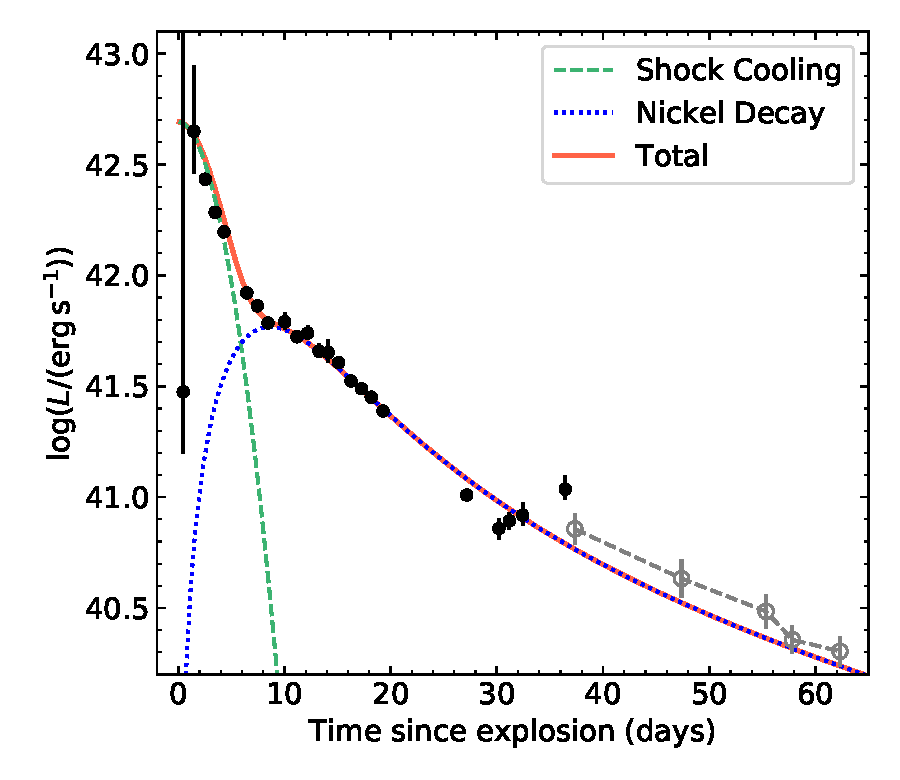
\includegraphics[width=\columnwidth]{figures/Lbb.pdf}
	\caption{Bolometric light curve for AT2019dge. The quasi-bolometric light curve of AT2019dge 
	estimated by computing $\nu L_\nu$ in $r$-band is shown as emply grey circles. The dashed green 
	and dotted blue lines show the best fits of shock cooling and nickel decay models. The solid red line 
	shows the combination of the two components.}
	\label{fig:Lbb}
\end{figure}

In Figure~\ref{fig:Lbb}, bolometric light curve measured in Section \ref{subsec:lc_properties} are shown 
in black. We also show late-time $r$-band $\nu L_{\nu}$ measurements in grey empty circles as a 
proxy of bolometric light curve evolution. The dashed green line  shows the best-fit model of 
$M_{\rm ext} = 9.34 \pm 0.36 \times 10^{-2} M_\odot$,
 $R_{\rm ext} =2.71_{-0.17}^{+0.19}\times10^{12}$\,cm (i.e., $39.0_{-2.5}^{+2.7} R_\odot$), 
 and first light epoch at phase $t_{\rm fl}= -3.21_\pm 0.04$\,day (i.e., the explosion occurred 0.45\,d 
 before the first detection in $g$-band). The amount of energy passed into the extended material is 
 well constrained to be $E_{\rm ext} = (1.15\pm 0.07) \times 10^{50}\,{\rm erg\, s^{-1}}$.

Given the simple assumptions of the model, we expect the constraints on $M_{\rm ext}$ and $R_{\rm 
ext}$ to be only approximatedly accurate. There are now numerous cases of early cooling envelope 
emission observed in CCSNe, where the extented matrial is estimated to have lower mass ($\sim 
0.001$--$0.01 M_\odot$) and larger radius ($\sim 10^{13}\, {\rm cm}$) compared to AT2019dge 
\citep{Modjaz2019}. We thus conclude that the early shock cooling emission was produced by an 
extended shell (instead of an envelope) with a mass of $\sim 0.1 M_\odot$ locating at a radius of $\sim 
3\times 10^{12}\,{\rm cm}$. 

\todo{try to see if puffier helium star produce lower ejecta mass. See eg Fig.16.7: Tauris 2003.
However, if it was really 50 Rsun at explosion, it would have been in such a wide binary that it could 
not have been 
stripped down to an envelope layer of just 0.3 Msun. This is quite intriguing! How sure are you of a 
progenitor 
radius of 50 Rsun? Could this radius instead represent some sort cocoon of helium-rich material 
ejected shortly 
before the SN? Even in the case of 14gqr, we saw that the star was too large (~ 500 Rsol) to explain a 
binary 
system stripped that much. We had explained this by invoking a short lived common envelope phase 
just before 
the explosion where the companion gets engulfed by the expanding He star. This could perhaps be the 
case here 
as well.}

\todo{rephrase: We conclude that the AT2019dge is not one of FELTs. Its fast $t_{\rm rise}$ is 
reminiscent of shock 
	cooling emission, and the moderate $t_{\rm decay}$ is consistent with coming from radioactivity.}

\begin{table}[!htbp] 
	\centering 
	\caption{shock P15.} 
	\begin{tabular}{ccll} 
		\hline 
		Name  &Type & $R_{\rm ext}$ ($10^{12}\,{\rm cm}$) & $M_{\rm ext}$ ($10^{-2} M_\odot$)  \\ 
		\hline
		iPTF16hgs & Ca-rich & $0.9$ & 8\\
		\textbf{AT2019dge} & Ib-pec & $2.69_{-0.16}^{+0.34}$ & $9.40_{-0.33}^{+0.69}$  \\
		iPTF14gqr & Ic-pec &$30^{+3}_{-3}$ &$0.88^{+0.08}_{-0.07}$  \\
		iPTF15dtg & Ic & 83&5 \\
		SN2016gkg & IIb &$4.00^{+0.05}_{-0.05}$ &$2.50^{+0.01}_{-0.01}$  \\
		ZTF18aalrxas & IIb & $73^{+3}_{-2}$  & $4.3_{-0.13}^{+0.14}$ \\
		\hline 
	\end{tabular} 
	\tablecomments{Reference: iPTF14gqr \citep{De2018}, SN2016gkg \citep{Arcavi2017}, 
		ZTF18aalrxas\citep{Fremling2019}}
\end{table} 


\subsection{Mass Loss Estimate from \ion{He}{II}} \label{subsec:flash}

 following the procedure given by \citet{Ofek2013} and \citet{De2018}, 
we use luminosity of the \ion{He}{II} $\lambda4686$ line to make an order-of-magnitude estimate on 
properties of the emission material. We get radius of the line emitting region $r \gtrsim 4.8 \times 
10^{13} \beta \,{\rm cm}$, mass losss parameter $K \gtrsim 1.2\times 10^{14} \, {\rm g\,cm^{-1}}$, and 
helium mass of the emitting region $M_{\rm He} \gtrsim 3.6\times 10^{-5} \beta^2\, M_{\odot}$, where 
$\beta$ is the ratio of the CSM width over radius. Note that these estimates can be affected if the CSM 
can not be well characterized by a spherically symmetric $\rho(r) \propto r^{-2}$ density profile, or if 
the emitting region was confined to a thin shell ($\beta \ll 1$).


Assuming that the CSM around the progenitor has a spherical wind-density profile of the form
$\rho = K r^{-2}$, where $r$ is distance from the progenitor, $K\equiv \dot M / (4\pi v_{\rm w})$ is the 
wind density parameter, $v_{\rm w}$ is the wind/outburst velocity, and $\dot M$ is the mass loss rate. 
The integrated mass of the emitting material from $r$ to $r_1$ is 
\begin{align}
M_{\rm He} = \int_{r}^{r_1}4\pi r^2 \rho(r) {\rm d}r=4\pi K \beta r
\end{align}
where $\beta \equiv (r_1 - r) /r $ is assumed to be of the order unity.

Following \citet{De2018}, we can relate the mass of the \ion{He}{II} region to the \ion{He}{II} 
$\lambda4686$ line luminosity using 
\begin{align}
L_{\lambda 4686} \approx \frac{A n_e M_{\rm He}}{m_{\rm He}} \label{eq:L4686}.
\end{align}
Here
\begin{align}
A = \frac{4\pi j_{\lambda 4686}}{n_e n_{\rm He^{++}}},
\end{align}
$ j_{\lambda4868}$ (in ${\rm erg \, cm^{-3}\, s^{-1}\, sr^{-1}}$) is the emission coefficient for the 
$\lambda4686$ transition. $m_{\rm He}$ is mass of a He nucleus, $n_{\rm He^{++}}$ is the number 
density of doubly ionized helium and $n_e$ is the number density of electrons.

Assuming a temperature of $10^4$\,K, electron density of $10^{10}\,{\rm cm^{-3}}$, and Case B 
recombination, we get $A=1.32\times 10^{-24}\,{\rm erg\, cm^{3}\, s^{-1}}$ \citep{Storey1995}. 
Assuming $n_e = 2 n_{\rm He^{++}}$ and using the density profile, Eq.~(\ref{eq:L4686}) can be written 
as
\begin{align}
L_{\lambda 4686} \approx \frac{8\pi A \beta}{m_{\rm He}^2} \frac{K^2}{r}.
\end{align}

The location of the emitting region can be constrained by requiring that the Thompson optical depth 
($\tau$) in the region must be small for the lines to escape. We require
\begin{align}
\tau = n_e \sigma_{\rm T} \int_{r}^{r_1} {\rm d}r = \frac{2\sigma_{\rm T}K\beta}{m_{\rm He}r} \lesssim 1
\end{align}
Thus
\begin{align}
r^2 &\gtrsim  \left (\frac{2\sigma_{\rm T}\beta}{m_{\rm He}} \right)^2 \frac{L_{\lambda 4686} m_{\rm 
		He}^2 r }{8\pi A \beta } \notag \\
r & \gtrsim L_{\lambda 4686} \frac{\sigma_{\rm T}^2  \beta }{2\pi A }
\end{align}

The $+0.4$\,d emission line flux is meausred to be $F = (8.37\pm 0.65)\times10^{-16}\,{\rm erg\, 
	cm^{-2}\,s^{-1}}$, correslonding to $L_{\lambda 4686} = 8.6\times 10^{38}\,{\rm erg\, s^{-1}}$. Hence, 
we get $r \gtrsim 4.8 \times 10^{13} \beta \,{\rm cm}$, $K \gtrsim 1.2\times 10^{14} \, {\rm 
	g\,cm^{-1}}$, and $M_{\rm He} \gtrsim 3.6\times 10^{-5} \beta^2\, M_{\odot}$.

\subsection{Constraints on Radio Emission}
\begin{figure}
	\centering
	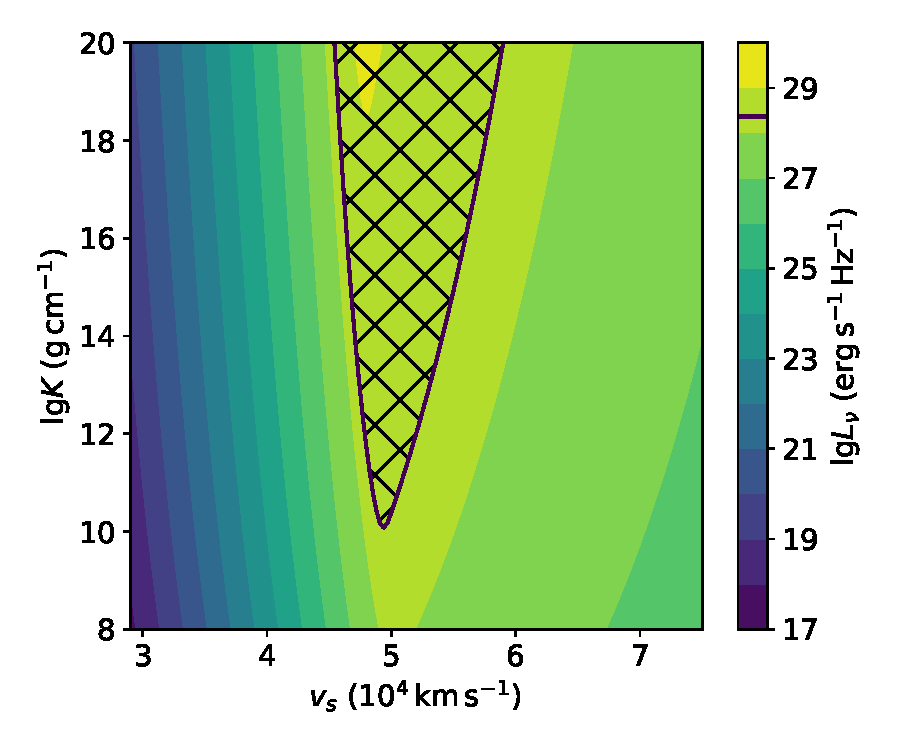
\includegraphics[width=\columnwidth]{figures/radio_230GHz_s2.pdf}
	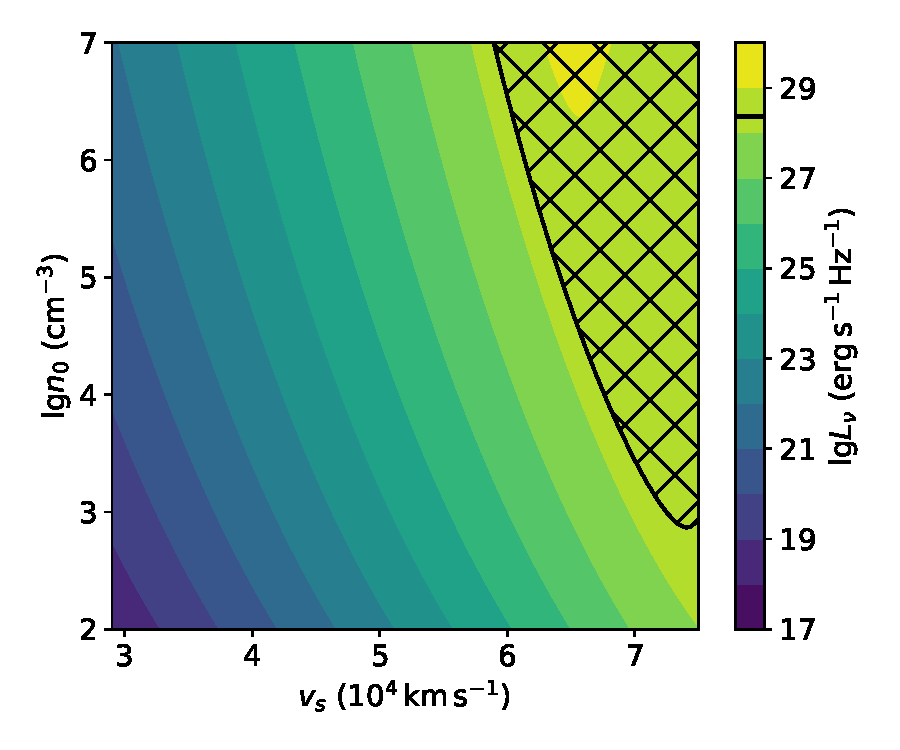
\includegraphics[width=\columnwidth]{figures/radio_230GHz_s0.pdf}
	\caption{Expected radio luminosity at 230\,GHz at different shock velocity $v_s$ and 
	wind mass-loss parameter $K$ in the case of $\rho \propto r^{-2}$ CSM environment (upper panel) 
	or number density $n_0$ in the constant-density case (bottom panel). The black contour in each 
	panel shows the location of the 3$\sigma$ upper limit at 230\,GHz on AT2019dge. The phase space 
	with a luminosity higher the black line in each panel is ruled out by the observation.
		\label{fig:radio}}
\end{figure}
Radio emission in SNe is produced by shock accelerated electrons in the circumstellar material as they 
gyrate in the post-shock magnetic field when the shock freely expands. Should the circumstellar 
medium be formed by a pre-SN stellar wind, the radio synchrotron radiation can be used to probe the 
pre-explosion mass-loss \citep{Chevalier1982}. High frequency ($\nu>90$\,GHz) bright 
($\nu L_\nu \gtrsim 10^{40} \, \rm erg\, 
s^{-1}$) radio sources are often found to be associated with gamma-ray bursts (GRBs), TDEs, and 
relativistic transients (see Figure~6 of \citealt{HoPhinney2019}). Among normal SNe Ibc, moderate 
submillimeter luminosity at $\sim 5\times 10^{37}\, \rm erg\, s^{-1}$ has been observed in SN1993J 
\citep{Weiler2007} and SN2011dh \citep{Horesh2013}.

Our SMA observations constrain the submillimeter luminosity of AT2019dge to $\nu L_{\nu \rm , 
230GHz} < 5.3\times 10^{39}\, \rm erg\, s^{-1}$ and $\nu L_{\nu \rm , 345GHz} < 3.0\times 10^{40}\, \rm 
erg\, s^{-1}$. Wwe place these upper limits in physical context using the synchrotron self-absorption 
model given by \citet{Chevalier1998}. The expected radio luminosities are computed at 230 and 
345\,GHz for two types of circumstellar environments --- one with the wind-density with the same 
parameterization as that adopted in Section \ref{subsec:flash} and the other with a constant-density 
environment ($\rho = \,{\rm constant}$). 

Adopting the explosion epoch found in Section \ref{subsec:fastrise}, our SMA observations were 
obtained at 2.75\,day after explosion. Given the early time of these observations, we consider constant 
shock velocities at 0.1--0.25$c$, as found to be typical in SNe Ibc \citep{Wellons2012}. We assume an 
electron energy power law index of $p = 3$, a volume filling factor $f=0.5$, and that the electrons 
and magnetic field in the post-shock region share constant fractions of the post-shock energy 
density, i.e., $\epsilon_e = \epsilon_B = 0.1$.

We show the contour plots (in the phase space of jet energy and circumstellar density) of the expected 
radio fluxes at the epochs of the VLA and GMRT observations for different viewing angles, along with 
our limits on the radio emission of this source in Figure 13. 
We constrain the wind mass-loss parameter $K$ and the external circumstellar density $n_0$ by 
obtaining the limiting cases for our 3$\sigma$ detections, as shown in Figure~\ref{fig:radio}.
xx in the wind-CSM case and xx in the constant-$\rho$ case

\subsection{Radioactivity Powered Main Peak}
After subtracting the shock cooling emission from the bolometric light curve, the remaining light curve 
has a peak luminosity of $L_{\rm peak}\approx 6\times 10^{41}\,{\rm erg \, s^{-1}}$ and a rise time of  
$t_{\rm peak}\approx 9\,{\rm d}$. In the shaded region of \citet[][Fig.~1]{Kasen2017}, this falls into the 
$M_{\rm Ni} = 0.1 M_{\rm ej}$ and $M_{\rm Ni} = 0.01 M_{\rm ej}$ lines, indicating that the remaining 
component can be powered by $^{56}$Ni decay. Here we use two methods to estimate $M_{\rm ej}$ 
and $M_{\rm Ni}$.

First of all, we use analytical models  \citep{Arnett1982, Valenti2008, Wheeler2015} to constrain the 
nickel mass ($M_{\rm Ni})$, a characteristic photon diffusion timescale ($\tau_{\rm m}$), and a 
characteristic $\gamma$-ray escape timescale ($t_0$). Details of the model fitting are illustrated in 
Appendix \ref{subsec:arnettfit}. The dotted blue line in Figure~\ref{fig:Lbb} shows the best-fit model of 
$M_{\rm Ni} = 1.69_{-0.04}^{+0.05}\times 10^{-2} M_\odot$, $\tau_{\rm m} = 7.15\pm 0.16$\,d, and $t_0 
= 22.17_{-0.73}^{+0.74}$\,d. Thus, using Equation~(\ref{eq:taum}), the ejecta mass can 
be estimated to be
\begin{align}
M_{\rm ej} = (0.46\pm 0.02) M_\odot \frac{v_{\rm ej}}{8150\,{\rm km\,s^{-1}}} \frac{0.07\,{\rm 
		cm^2\,g^{-1}}}{\kappa_{\rm 	opt}} \notag
\end{align}

Recently, \citet[][hereafter KK19]{Khatami2019} presents improved analytic relations (compared with 
the original \citealt{Arnett1982} model) between $t_{\rm peak}$ and $L_{\rm peak}$. When $t<10$\,d, 
$\varepsilon_{\rm Ni}(t) \gg \varepsilon_{\rm Co}(t)$ (see Equations~\ref{eq:heatNi}, \ref{eq:heatCo}), 
and thus we have an exponential heating function 
\begin{equation}
L_{\rm heat}(t) = L_0 e^{-t/\tau_{\rm Ni}}
\end{equation}
where $L_0 = M_{\rm Ni}\times \epsilon_{\rm Ni}$. In this case, KK19 (Eq.~21) shows that 
the relation between peak time and luminosity is:
\begin{equation}
L_{\rm peak} = \frac{2L_0 \tau_{\rm Ni}^2}{\beta^2 t_{\rm peak}^2} \left[ 1 - (1 + \beta t_{\rm 
peak}/\tau_{\rm Ni} ) e^{-\beta t_{\rm peak}/ \tau_{\rm Ni}} \right]
\end{equation}
where $\beta \sim 4/3$ gives a reasonable match to numerical simulations. With $L_{\rm 	peak}\approx 
6\times 10^{41}\,{\rm erg \, s^{-1}}$ and $t_{\rm peak} \approx 9$\,d, we get an estimate of $M_{\rm 
Ni}\sim 0.018 M_{\odot}$. 

$M_{\rm ej}$ can be estimated using Eq.~23 of KK19:
\begin{align}
\frac{t_{\rm peak}}{t_{\rm d}} = 0.11\,{\rm ln} \left( 1 + \frac{9\tau_{\rm Ni}}{t_{\rm d}} \right)+ 0.36,
\label{eq:kk19_23}
\end{align}
where $t_{\rm d}$ is the characteristic timescale without any numerical factors
\begin{align}
t_{\rm d} = \left(\frac{\kappa_{\rm opt} M_{\rm ej}}{v_{\rm ej}c}\right)^{1/2}. \label{eq:kk19_12}
\end{align}
We derive $t_{\rm d} \approx 16.2$\,d, which implies 
\begin{align}
M_{\rm ej} \approx 0.30 M_\odot \frac{v_{\rm ej}}{8150\,{\rm km\,s^{-1}}} \frac{0.07\,{\rm 
		cm^2\,g^{-1}}}{\kappa_{\rm 	opt}} \notag
\end{align}

In conclusion, the estimates derived from simplified modelling fitting and new analytic relations from 
KK19 are roughly the same. Ejecta mass and nickle mass from the explosion of AT2019dge are very 
small, $M_{\rm ej}\sim 0.3M_\odot$, $M_{\rm Ni} \sim 0.02M_\odot$.

\subsection{A Highly Stripped Progenitor in a Binary System}
The shock cooling powered early emission followed by the radioactivity powered decay indicates that 
AT2019dge is associated with the class of iron core-collapse events. The small amout of ejecta 
mass requires extreme stripping prior to the explosion, and rules out single massive star to be the 
progenitor. The helium-rich photosperic phase spectra suggests that the bulk of the ejecta should be 
helium.

The evolution of binary massive stars

Tight helium star--NS binary systems, presumably created in the common-envelope phase from 
high-mass X-ray binaries, can lead to the extrame stripping of the helium envelope pand result in SNe 
with ejecta masses of the order of 0.1Msun 

Many progenitors are expected to have a helium mass above the critical helium mass (0.1 Msun, 
Hachingerr 2012) required to observe optical helium features Tauris 2015 and thus may be observed as 
SN Ib like AT2019dge.

In this picture, the helium-star mass transfer rate is 3--4 orders of magnitude greater than the 
Eddington accretion rate  for NSs and $>99.9$\% of the transferred mass is lost from the system 
\citep{Tauris2015}, forming a shell of $\sim 0.1 M_\odot$ and $3\times 10^{12}\,{\rm cm}$ at the time of 
explosion.

\todo{This is actually not ultra-stripped SN: Mej larger than 0.2 Msun. Can form this using HMLB -- 
Case BB RLO -- stripp -- double NS.  OR. Massive star explosion??}

\section{Discussion}

\citet{Woosley2019} shows that mass-losing helium stars with initial masses between 2.5--3.2 
$M_\odot$ experience raidus expansion after helium depletion (but lack a strong silicon flash), which 
gives rise to the early-time shock 
cooling emission out of the ejected helium envelope. If the explosion makes substantial $^{56}$Ni, then 
the light curve may have two peaks, the second resembling a SN Ib but occurring earlier due to the low 
$M_{\rm ej}$.


\todo{ask Thomas: discussions on the age of the system (e.g. the time to the 2nd SN in a binary 
system in relation 
to a star burst in the host galaxy, and a few words on the subsequent delay time until a merger - in 
case 
AT2019dge represents an event where it is the 2nd SN producing a double compact object binary that 
remains 
bound).}

massive mass-loss episode that takes place just prior to the explosion \citep{Shiode2014}

Progenitor: why so rare???
Could the progenitor be a helium rich WR star, perhaps recently transitioned from an LBV phase 

Constraints on event rate?



\section{Conclusion}
In this paper we have presented observations and modeling of the fast transient AT2019dge. We 
summarize our primary observational findings below:
\begin{enumerate}[label=(\alph*)]
	\item Peak absolute magnitude of MB = −dd mag and decline parameter of hah mag.
	\item  Total Nickel and ejecta masses of $M_{\rm Ni} = 0.02 \pm 0.01$ and $Mej = 0.3 \pm 0.3 
	M_\odot$, respectively.
	\item spectrum is peculiar
	\item photosperic phase spec emission comes from a photosphere receding (in mass coordinates) 
	back through freely expanding SN ejecta (smith 2016 rewrite)
	\item Ca-rich event nebular spectrum
\end{enumerate}

equatorial CSM deposited by binary interaction (Smith2017)


The combination of depth, cadence and sky coverage offered by ongoing time domain surveys enables 
detection within one day of the explosion, opening a new window into the relatively unexplored early 
phase of these events. 

Enhanced (and potentially eruptive) mass-loss during the final stages of stellar evolution is a key probe 
of poorly understood physics (e.g., Shiode \& Quataert 2013; Smith \& Arnett 2014) that sets the initial 
conditions to core-collapse. 

Despite the steady increase in the number of events in the class of sub-luminous transients, the total 
number of well-studied events remain still small ($\approx 10$). An all-sky two-day cadence survey 
with ZTF Phase II is ideally positioned to probe this rare population over a sufficiently large volume 
(given the deeper limiting magnitude of ZTF compared to other ongoing time domain surveys) to 
address questions regarding their intrinsic properties such as luminosity functions, spectroscopic 
diversity and ejecta mass distributions of the different sub-types and their volumetric rates. As likely 
tracers of the end points of white dwarfs and massive stars in extreme binary systems, their intrinsic 
rates are not only important from the point of view of understanding these rare transient phenomena 
but also have direct implications for current and future experiments in the field of gravitational wave 
astronomy. With a higher cadence than the nominal 3-day public survey in Phase I, the 2-day cadence 
in $g$ and $r$ bands will be particularly sensitive to the population of fastest transients in the local 
universe, of which only a handful are known, while the two-color coverage will also be a powerful 
diagnostic of the intrinsic color of these events.

wide-field 
optical surveys. 

disminutive

see helium -- less stripped compared with iPTF14gqr


\acknowledgements

%% Y. Yao thanks the instructors and organisers of the GROWTH summer school for teaching 
%%essential skills in time-domain data analysis.
%% discussion with Wenbin Lu, Udi Nakar, Nathan Smith, Yan Lin, Christoffer, Fremling, Avishay
%% Jim, Sterl, Tony
This study made use of the open supernova catalog \citep{Guillochon2017}.

This work was supported by the GROWTH project funded by the National Science Foundation under 
PIRE grant No.\,1545949. 

This work is based on observations obtained with the Samuel Oschin Telescope 48 inch and the 60 
inch Telescope at the Palomar Observatory as part of the Zwicky Transient Facility project. ZTF is 
supported by the National Science Foundation under grant No. AST-1440341 and a collaboration 
including Caltech, IPAC, the Weizmann Institute for Science, the Oskar Klein Center at Stockholm 
University, the University of Maryland, the University of Washington, Deutsches 
Elektronen-Synchrotron and Humboldt University, Los Alamos National Laboratories, the TANGO 
Consortium of Taiwan, the University of Wisconsin at Milwaukee, and Lawrence Berkeley National 
Laboratories. Operations are conducted by COO, IPAC, and UW. 

\software{
          \texttt{astropy} \citep{Astropy-Collaboration2013},
          \texttt{scipy} \citep{Jones2001}, 
          \texttt{matplotlib} \citep{Hunter2007},
          \texttt{pandas} \citep{McKinney2010},
          \texttt{emcee} \citep{Foreman-Mackey2013},
          \texttt{corner} \citep{Foreman-Mackey2016},
          \texttt{pyneb} \citep{Luridiana2013}
          }

%% For this sample we use BibTeX plus aasjournals.bst to generate the
%% the bibliography. The sample63.bib file was populated from ADS. To
%% get the citations to show in the compiled file do the following:
%%
%% pdflatex sample63.tex
%% bibtext sample63
%% pdflatex sample63.tex
%% pdflatex sample63.tex

\clearpage
\appendix

\section{UV and Optical Photometry} \label{sec:appphot}
\subsection{Data}\label{subsec:appphot_data}
\startlongtable
\begin{deluxetable}{llllll}
\tabletypesize{\scriptsize}
\tablecaption{Optical and UV photometry for AT2019dge.\label{tab:phot}}
\tablehead{
\colhead{Date (JD)}   
& \colhead{Instrument}
& \colhead{Filter}  
& \colhead{$m$} 
& \colhead{$\sigma_{m}$}
}
\startdata
58582.1544 & LT$+$IOO & $g$ & 18.59 & 0.01 \\
58582.1552 & LT$+$IOO & $r$ & 18.84 & 0.02 \\
58582.1575 & LT$+$IOO & $i$ & 19.11 & 0.02 \\
58582.1583 & LT$+$IOO & $z$ & 19.28 & 0.07 \\
58583.1637 & LT$+$IOO & $g$ & 18.48 & 0.02 \\
58583.1645 & LT$+$IOO & $r$ & 18.63 & 0.01 \\
58584.2324 & LT$+$IOO & $g$ & 18.58 & 0.01 \\
58584.2332 & LT$+$IOO & $r$ & 18.68 & 0.02 \\
58584.2355 & LT$+$IOO & $i$ & 18.85 & 0.02 \\
58584.2363 & LT$+$IOO & $z$ & 19.15 & 0.07 \\
58590.0252 & LT$+$IOO & $g$ & 19.47 & 0.14 \\
58590.0260 & LT$+$IOO & $r$ & 19.16 & 0.04 \\
58590.0268 & LT$+$IOO & $i$ & 19.24 & 0.07 \\
58590.0277 & LT$+$IOO & $z$ & 19.28 & 0.21 \\
58591.0676 & LT$+$IOO & $g$ & 19.44 & 0.07 \\
58591.0685 & LT$+$IOO & $r$ & 19.31 & 0.09 \\
58591.0693 & LT$+$IOO & $i$ & 19.22 & 0.06 \\
58591.0701 & LT$+$IOO & $z$ & 19.10 & 0.12 \\
58592.0472 & LT$+$IOO & $g$ & 19.40 & 0.13 \\
58592.0472 & LT$+$IOO & $r$ & 19.26 & 0.12 \\
58592.0489 & LT$+$IOO & $i$ & 19.27 & 0.10 \\
58592.0497 & LT$+$IOO & $z$ & 19.33 & 0.17 \\
58593.1109 & LT$+$IOO & $r$ & 19.41 & 0.06 \\
58593.1117 & LT$+$IOO & $i$ & 19.41 & 0.08 \\
58593.1125 & LT$+$IOO & $z$ & 19.46 & 0.12 \\
58594.1142 & LT$+$IOO & $g$ & 19.69 & 0.20 \\
58594.1150 & LT$+$IOO & $r$ & 19.50 & 0.08 \\
58594.1158 & LT$+$IOO & $i$ & 19.48 & 0.08 \\
58594.1167 & LT$+$IOO & $z$ & 19.52 & 0.16 \\
58595.0926 & LT$+$IOO & $g$ & 19.82 & 0.10 \\
58595.0935 & LT$+$IOO & $r$ & 19.60 & 0.07 \\
58595.0943 & LT$+$IOO & $i$ & 19.45 & 0.07 \\
58595.0951 & LT$+$IOO & $z$ & 19.55 & 0.11 \\
58596.1380 & LT$+$IOO & $g$ & 20.10 & 0.11 \\
58596.1388 & LT$+$IOO & $r$ & 19.75 & 0.06 \\
58596.1396 & LT$+$IOO & $i$ & 19.66 & 0.08 \\
58596.1405 & LT$+$IOO & $z$ & 19.71 & 0.16 \\
58597.1508 & LT$+$IOO & $g$ & 20.12 & 0.07 \\
58597.1516 & LT$+$IOO & $r$ & 19.77 & 0.05 \\
58597.1539 & LT$+$IOO & $i$ & 19.69 & 0.07 \\
58597.1547 & LT$+$IOO & $z$ & 19.95 & 0.15 \\
58598.1207 & LT$+$IOO & $g$ & 20.37 & 0.17 \\
58598.1218 & LT$+$IOO & $r$ & 19.89 & 0.06 \\
58598.1247 & LT$+$IOO & $i$ & 19.73 & 0.08 \\
58598.1257 & LT$+$IOO & $z$ & 20.13 & 0.30 \\
58599.1894 & LT$+$IOO & $g$ & 20.42 & 0.08 \\
58599.1918 & LT$+$IOO & $z$ & 20.17 & 0.12 \\
58601.1606 & LT$+$IOO & $i$ & 20.38 & 0.10 \\
58607.0861 & LT$+$IOO & $r$ & 21.22 & 0.11 \\
58607.0890 & LT$+$IOO & $i$ & 20.88 & 0.10 \\
58607.0900 & LT$+$IOO & $z$ & 20.72 & 0.16 \\
58610.1965 & LT$+$IOO & $g$ & 21.86 & 0.19 \\
58610.1974 & LT$+$IOO & $r$ & 21.36 & 0.21 \\
58610.1982 & LT$+$IOO & $i$ & 21.28 & 0.19 \\
58610.1990 & LT$+$IOO & $z$ & 20.92 & 0.42 \\
58611.1743 & LT$+$IOO & $g$ & 21.77 & 0.23 \\
58611.1751 & LT$+$IOO & $r$ & 21.52 & 0.19 \\
58611.1759 & LT$+$IOO & $i$ & 21.10 & 0.12 \\
58611.1767 & LT$+$IOO & $z$ & 20.72 & 0.21 \\
58580.4421 & P48$+$ZTF & $g$ & 20.83 & 0.15 \\
58581.4807 & P48$+$ZTF & $g$ & 18.81 & 0.03 \\
58582.4396 & P48$+$ZTF & $g$ & 18.50 & 0.02 \\
58583.4082 & P48$+$ZTF & $g$ & 18.52 & 0.04 \\
58584.4691 & P48$+$ZTF & $g$ & 18.65 & 0.02 \\
58586.4480 & P48$+$ZTF & $g$ & 19.04 & 0.02 \\
58587.4658 & P48$+$ZTF & $g$ & 19.18 & 0.03 \\
58588.4794 & P48$+$ZTF & $g$ & 19.39 & 0.04 \\
58591.3740 & P48$+$ZTF & $g$ & 19.68 & 0.15 \\
58592.4784 & P48$+$ZTF & $g$ & 19.50 & 0.10 \\
58593.4841 & P48$+$ZTF & $g$ & 19.78 & 0.17 \\
58596.4781 & P48$+$ZTF & $g$ & 20.11 & 0.08 \\
58597.4728 & P48$+$ZTF & $g$ & 20.53 & 0.18 \\
58599.2766 & P48$+$ZTF & $g$ & 20.47 & 0.08 \\
58612.4016 & P48$+$ZTF & $g$ & 21.78 & 0.22 \\
58616.4688 & P48$+$ZTF & $g$ & 21.66 & 0.16 \\
58580.4842 & P48$+$ZTF & $r$ & 20.89 & 0.14 \\
58581.4308 & P48$+$ZTF & $r$ & 19.19 & 0.05 \\
58582.4516 & P48$+$ZTF & $r$ & 18.76 & 0.02 \\
58584.4009 & P48$+$ZTF & $r$ & 18.69 & 0.02 \\
58585.4191 & P48$+$ZTF & $r$ & 18.75 & 0.03 \\
58586.4101 & P48$+$ZTF & $r$ & 18.92 & 0.03 \\
58587.4222 & P48$+$ZTF & $r$ & 19.02 & 0.05 \\
58588.4300 & P48$+$ZTF & $r$ & 19.10 & 0.03 \\
58589.3489 & P48$+$ZTF & $r$ & 18.99 & 0.20 \\
58591.4525 & P48$+$ZTF & $r$ & 19.31 & 0.05 \\
58592.3880 & P48$+$ZTF & $r$ & 19.46 & 0.13 \\
58593.4315 & P48$+$ZTF & $r$ & 19.44 & 0.06 \\
58596.3929 & P48$+$ZTF & $r$ & 19.68 & 0.05 \\
58597.4050 & P48$+$ZTF & $r$ & 19.85 & 0.06 \\
58598.3610 & P48$+$ZTF & $r$ & 19.96 & 0.09 \\
58599.4846 & P48$+$ZTF & $r$ & 19.97 & 0.06 \\
58600.4715 & P48$+$ZTF & $r$ & 20.08 & 0.10 \\
58605.4333 & P48$+$ZTF & $r$ & 20.73 & 0.08 \\
58607.3705 & P48$+$ZTF & $r$ & 20.69 & 0.09 \\
58608.4033 & P48$+$ZTF & $r$ & 20.64 & 0.13 \\
58612.4549 & P48$+$ZTF & $r$ & 21.23 & 0.11 \\
58616.4117 & P48$+$ZTF & $r$ & 20.94 & 0.09 \\
58617.3380 & P48$+$ZTF & $r$ & 21.02 & 0.17 \\
58627.3911 & P48$+$ZTF & $r$ & 21.58 & 0.21 \\
58635.3518 & P48$+$ZTF & $r$ & 21.95 & 0.19 \\
58581.5163 & P48$+$ZTF & $i$ & 19.44 & 0.17 \\
58586.5159 & P48$+$ZTF & $i$ & 18.98 & 0.08 \\
58596.3822 & P48$+$ZTF & $i$ & 19.66 & 0.16 \\
58637.8263 & P48$+$ZTF & $r$ & 22.27 & 0.16 \\
58642.3119 & P48$+$ZTF & $r$ & 22.40 & 0.17 \\
58582.8289 & $Swift+$UVOT & $B$ & 18.68 & 0.40 \\
58582.8280 & $Swift+$UVOT & $U$ & 18.80 & 0.10 \\
58582.8346 & $Swift+$UVOT & $UVM2$ & 18.55 & 0.07 \\
58582.8261 & $Swift+$UVOT & $UVW1$ & 18.61 & 0.19 \\
58582.8299 & $Swift+$UVOT & $UVW2$ & 18.68 & 0.11 \\
58582.8337 & $Swift+$UVOT & $V$ & 18.29 & 0.11 \\
58583.5775 & $Swift+$UVOT & $B$ & 18.46 & 0.29 \\
58583.5766 & $Swift+$UVOT & $U$ & 19.22 & 0.10 \\
58583.5833 & $Swift+$UVOT & $UVM2$ & 18.85 & 0.09 \\
58583.5747 & $Swift+$UVOT & $UVW1$ & 18.49 & 0.14 \\
58583.5785 & $Swift+$UVOT & $UVW2$ & 18.87 & 0.10 \\
58583.5823 & $Swift+$UVOT & $V$ & 18.51 & 0.11 \\
\enddata
\tablecomments{$m$ and $\sigma_m$ are observed magnitude (without extinction correction) in AB system.}
\end{deluxetable}

\begin{deluxetable}{llll}[htbp!]
		\tabletypesize{\scriptsize}
		\tablecaption{Photometry of the host galaxy \label{tab:host_phot}}
		\tablehead{
\colhead{Instrument/Filter}
& \colhead{$\lambda_{\rm eff}$ ($\rm \AA$)}
& \colhead{$m$}
& \colhead{$\sigma_{m}$}
	}
\startdata
% UVOT checked (lambda_eff, mag, emag)
UVOT/$UVW2$ 		& 2079.0  & 20.492 & 0.124\\
UVOT/$UVM2$		& 2255.1  &  20.471 & 0.172\\
UVOT/$UVW1$ 		& 2614.2  &  20.081  & 0.155\\
UVOT/$U$		& 3475.5  &  19.631 & 0.145\\
UVOT/$B$		& 4359.1  &  18.812 & 0.139\\
UVOT/$V$		& 5430.1  &  18.194  & 0.171\\
% SDSS checked (lambda_eff, mag, emag)
SDSS/$u'$ 		& 3561.8  &  19.636	& 0.082	\\
SDSS/$g'$ 		& 4718.9  &  18.540 & 0.015	\\
SDSS/$r'$ 		& 6185.2  & 18.056	 & 0.026 \\
SDSS/$i'$ 		& 7499.7     &17.885 & 0.028\\
SDSS/$z'$ 		& 8961.5     &17.697 & 0.089\\
% PS1 checked (lambda_eff, mag, emag)
PS1/$g_{\rm PS1}$	& 4866.5     & 18.538 & 0.042\\
PS1/$r_{\rm PS1}$	& 6214.6     & 18.029  & 0.030\\
PS1/$i_{\rm PS1}$	& 7544.6     &17.845 &0.033\\
PS1/$z_{\rm PS1}$	& 8679.5     & 17.755 & 0.050\\
PS1/$y_{\rm PS1}$	& 9633.3     &17.710  & 0.063\\
% 2MASS
2MASS/$J$ 		& 12410.5   & 17.653 & 0.215\\
2MASS/$H$ 		& 16513.7   &17.690 & 0.420\\
% WISE
WISE/$W1$ 		& 34002.6    & 18.460 & 0.069\\
WISE/$W2$   & 46520.1    & 18.953 &  0.136\\
\enddata
\tablecomments{$m$ and $\sigma_m$ are observed magnitude (without extinction correction) in the AB 
system.
}
\end{deluxetable}
	

The full set of photometry of AT2019dge is listed in Table~\ref{tab:phot}. Photometry of the host 
galaxy SDSS J173646.73+503252.3 is listed in Table~\ref{tab:host_phot}.

In Figure \ref{fig:seds} we show the photometry interpolated onto common epochs, and fit to a 
blackbody function to derive the photospheric evolution (see Section \ref{subsec:lc_properties}). The 
resulting evolution in bolometric lumonosity, photospheric radius, and effective temperatures is listed 
in Table  \ref{tab:bbfit}
\begin{figure*}
    \centering
    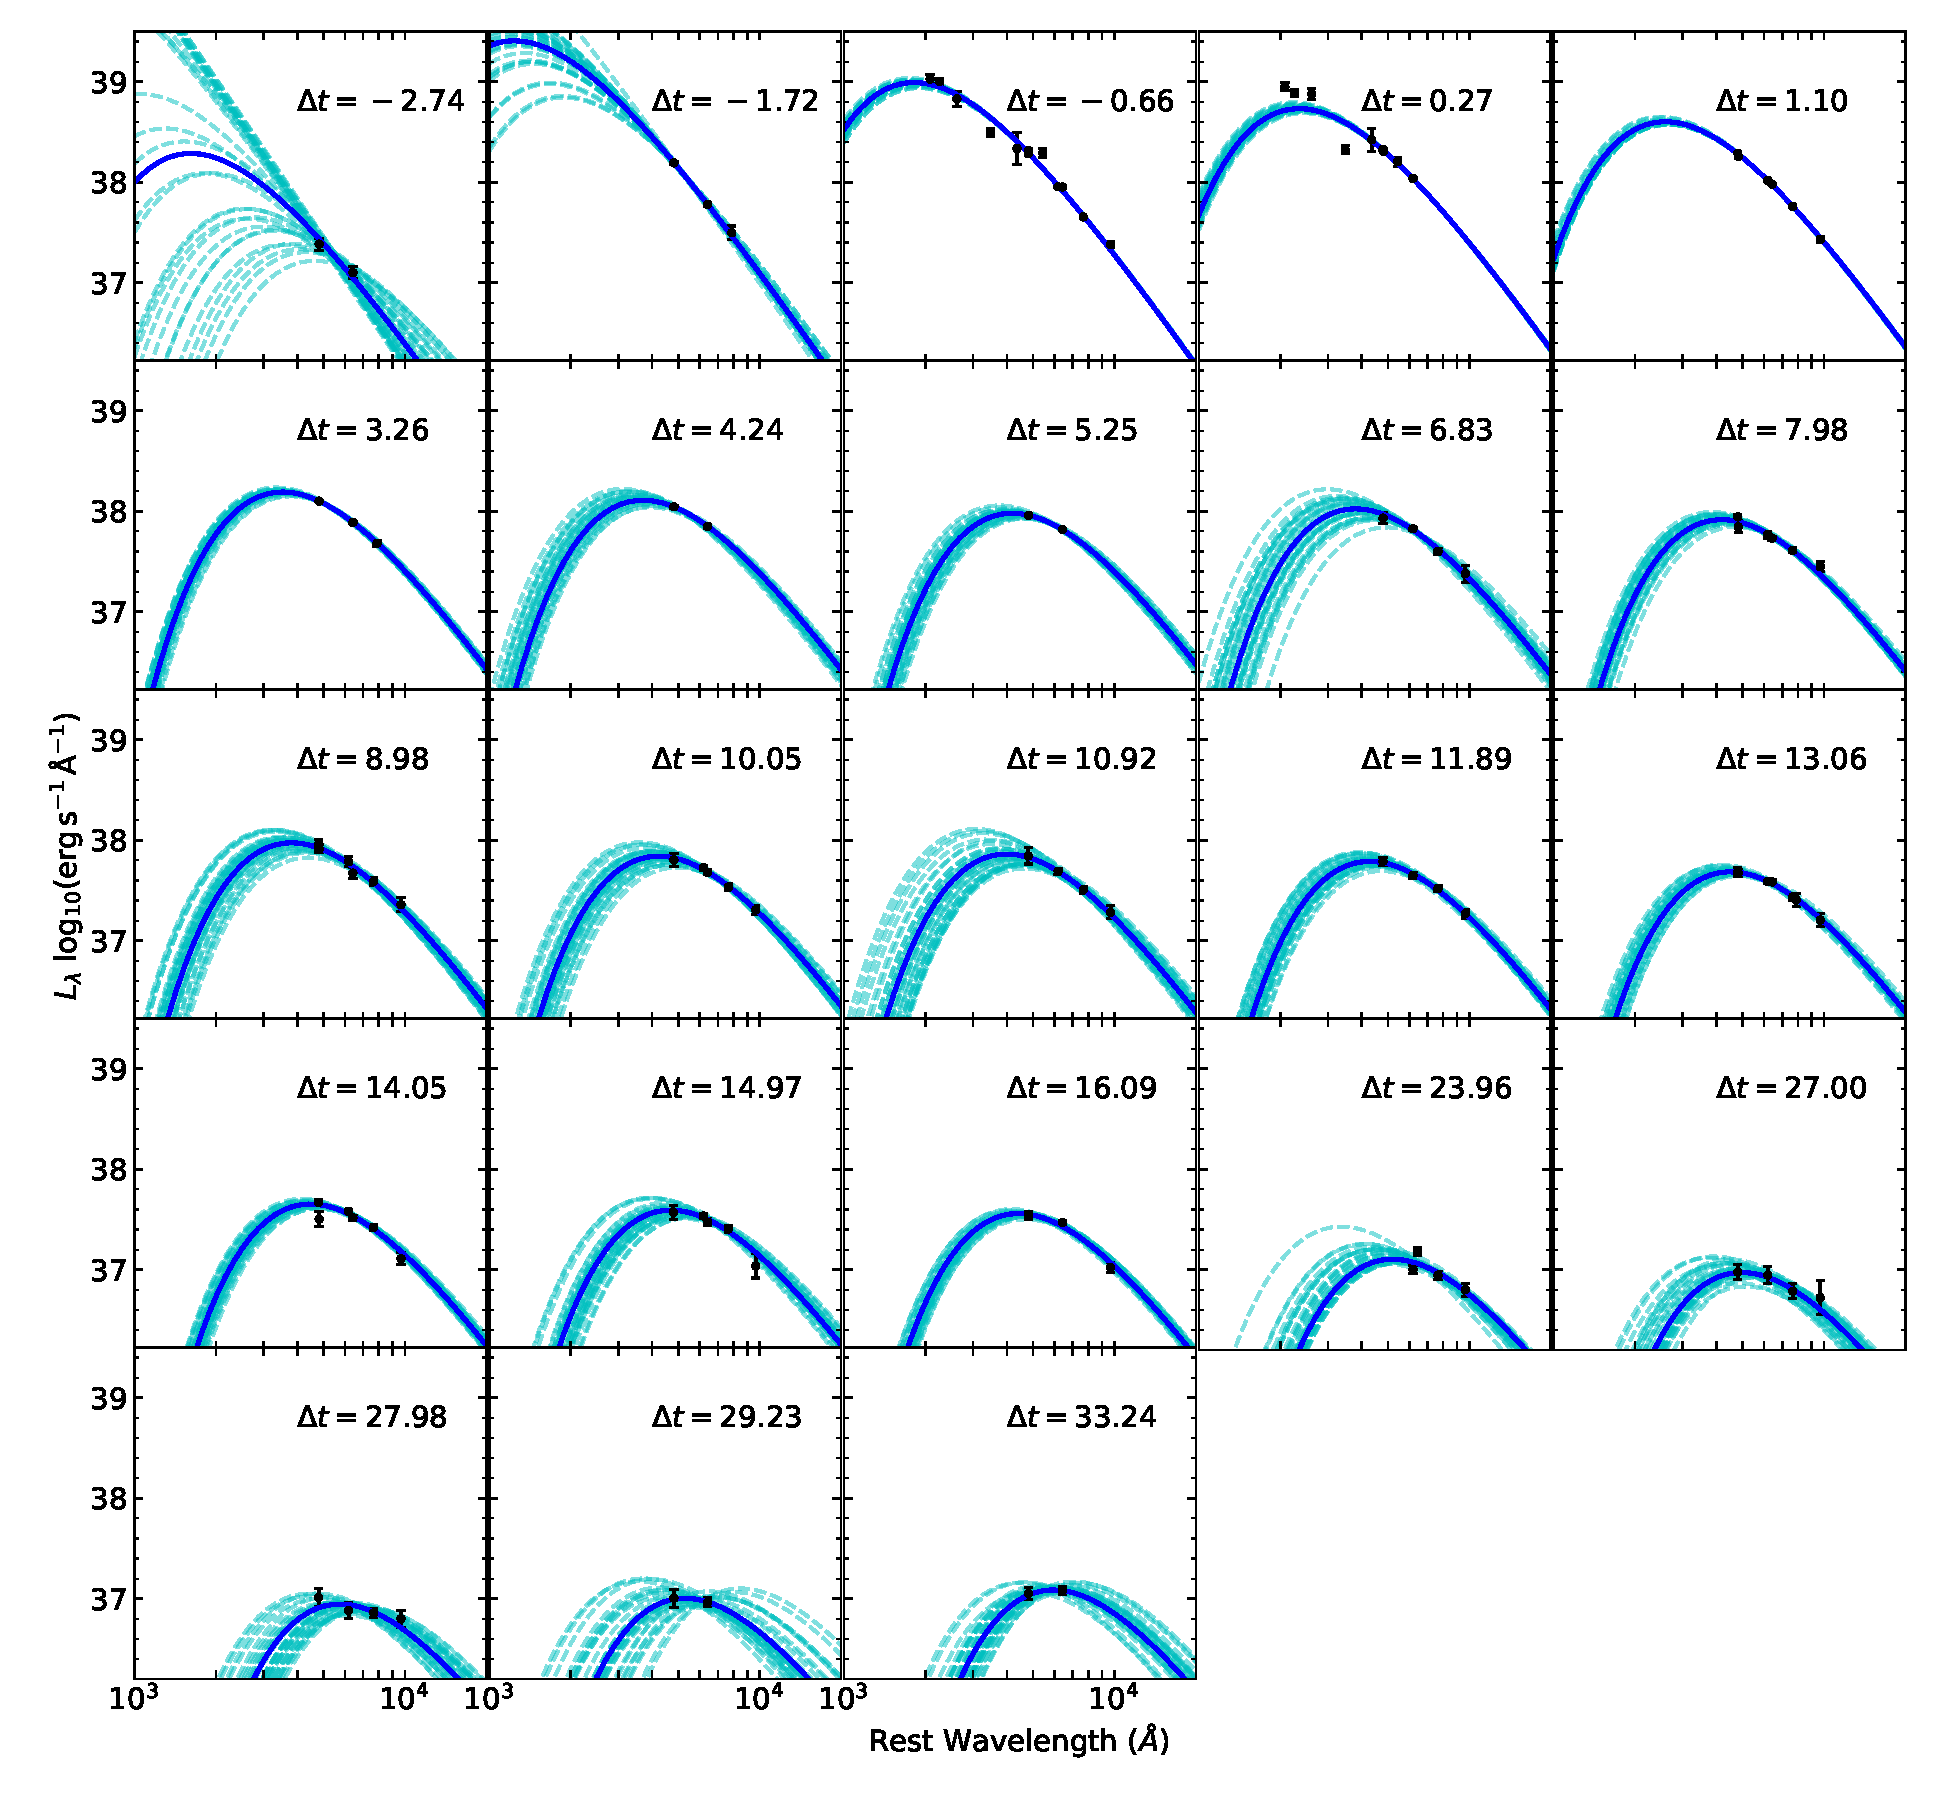
\includegraphics[width = 0.9\textwidth]{figures/seds.pdf}
    \caption{Black data points are $Swift$/UVOT and optical photometry of AT2019dge. Solid lines show 
    the maximum MCMC a posteriori model fits. Dashed lines are simple $\chi^2$ fits. 
    \label{fig:seds}}
\end{figure*}
\begin{table}[!htbp] 
	\centering 
	\caption{Physical evolution of SN2019dge from blackbody fits.} 
	\begin{tabular}{lrrr} 
		\hline 
		$\Delta t$ & $L (10^{41} \,{\rm erg\,s^{-1}})$ & $R$ ($10^{3}\,R_\odot$) & $T$ ($10^3$\,K) \\ 
		\hline
		-2.74 & $2.98^{+578.84}_{-1.41}$ &$1.45^{+1.14}_{-1.14}$ &$14.21^{+101.35}_{-5.12}$  \\
		-1.72 & $44.63^{+43.85}_{-15.84}$ &$2.20^{+0.44}_{-0.46}$ &$22.75^{+7.60}_{-4.14}$  \\
		-0.66 & $27.15^{+1.13}_{-1.07}$ &$3.48^{+0.08}_{-0.08}$ &$15.96^{+0.34}_{-0.33}$  \\
		0.27 & $19.26^{+0.77}_{-0.72}$ &$4.92^{+0.14}_{-0.14}$ &$12.32^{+0.29}_{-0.28}$  \\
		1.10 & $15.72^{+0.46}_{-0.42}$ &$5.39^{+0.14}_{-0.14}$ &$11.20^{+0.23}_{-0.22}$  \\
		3.26 & $8.34^{+0.22}_{-0.20}$ &$7.26^{+0.46}_{-0.44}$ &$8.23^{+0.31}_{-0.28}$  \\
		4.24 & $7.29^{+0.26}_{-0.22}$ &$7.38^{+0.88}_{-0.83}$ &$7.88^{+0.54}_{-0.46}$  \\
		5.25 & $6.10^{+0.16}_{-0.15}$ &$8.77^{+0.78}_{-0.73}$ &$6.92^{+0.33}_{-0.30}$  \\
		6.83 & $6.18^{+0.63}_{-0.46}$ &$7.09^{+1.01}_{-0.92}$ &$7.72^{+0.75}_{-0.62}$  \\
		7.98 & $5.29^{+0.24}_{-0.21}$ &$8.00^{+0.75}_{-0.70}$ &$6.99^{+0.39}_{-0.35}$  \\
		8.98 & $5.49^{+0.44}_{-0.36}$ &$6.79^{+0.94}_{-0.85}$ &$7.66^{+0.65}_{-0.56}$  \\
		10.05 & $4.55^{+0.37}_{-0.27}$ &$7.42^{+1.03}_{-0.96}$ &$6.99^{+0.63}_{-0.52}$  \\
		10.92 & $4.49^{+0.64}_{-0.44}$ &$6.63^{+1.25}_{-1.06}$ &$7.37^{+0.93}_{-0.75}$  \\
		11.89 & $4.04^{+0.24}_{-0.21}$ &$7.42^{+0.83}_{-0.75}$ &$6.79^{+0.45}_{-0.40}$  \\
		13.06 & $3.34^{+0.10}_{-0.10}$ &$7.52^{+0.69}_{-0.66}$ &$6.43^{+0.32}_{-0.29}$  \\
		14.05 & $3.08^{+0.10}_{-0.09}$ &$7.05^{+0.63}_{-0.59}$ &$6.51^{+0.32}_{-0.29}$  \\
		14.97 & $2.82^{+0.15}_{-0.12}$ &$7.30^{+1.21}_{-1.06}$ &$6.25^{+0.57}_{-0.49}$  \\
		16.09 & $2.45^{+0.09}_{-0.09}$ &$6.17^{+0.59}_{-0.58}$ &$6.56^{+0.33}_{-0.29}$  \\
		23.96 & $1.02^{+0.07}_{-0.06}$ &$5.47^{+1.23}_{-1.12}$ &$5.59^{+0.74}_{-0.54}$  \\
		27.00 & $0.72^{+0.08}_{-0.08}$ &$4.08^{+1.26}_{-1.01}$ &$5.93^{+0.91}_{-0.70}$  \\
		27.98 & $0.78^{+0.07}_{-0.06}$ &$5.73^{+1.68}_{-1.29}$ &$5.10^{+0.68}_{-0.57}$  \\
		29.23 & $0.83^{+0.11}_{-0.09}$ &$4.76^{+2.47}_{-1.56}$ &$5.64^{+1.23}_{-0.93}$  \\
		33.24 & $1.09^{+0.16}_{-0.11}$ &$6.99^{+2.47}_{-1.74}$ &$5.02^{+0.65}_{-0.56}$  \\
		\hline 
	\end{tabular} 
	\label{tab:bbfit} 
\end{table} 


\subsection{Modelling Early Light Curve} \label{subsec:p15fit}
\begin{deluxetable}{llc}[htpb!]
	\tablecaption{Shock cooling model parameters $\theta$ and their priors \label{tab:P15priors}}
	\tablehead{
		\colhead{$\theta$}
		& \colhead{Description}
		&\colhead{Prior}
	}
	\startdata
	${\rm log}R_{\rm ext}$ & log$_{10}$ of extented material radius in cm  & 
	$\mathcal{U}(-5, 25)$ \\
	${\rm log}M_{\rm ext}$ &  log$_{10}$ of extented material mass in $M_\odot$  & $\mathcal{U}(-4, 
	0)$\\
	$t_\mathrm{exp}$ & explosion epoch in MJD relative to $58583.2$& $\mathcal{U}(-8,-2.76)$ \\
	$E_{51}$ & SN energy divided by $10^{51}\,{\rm erg}$ & $\mathcal{U}(0.01, 10)$ \\
	$E_{\rm ext, 49}$ & $E_{\rm ext}$ divided by $10^{49}\,{\rm erg}$ & 
	$\mathcal{U}(0.1,100)$ \\
	\enddata
\end{deluxetable}



\begin{figure}[htbp!]
	\centering
	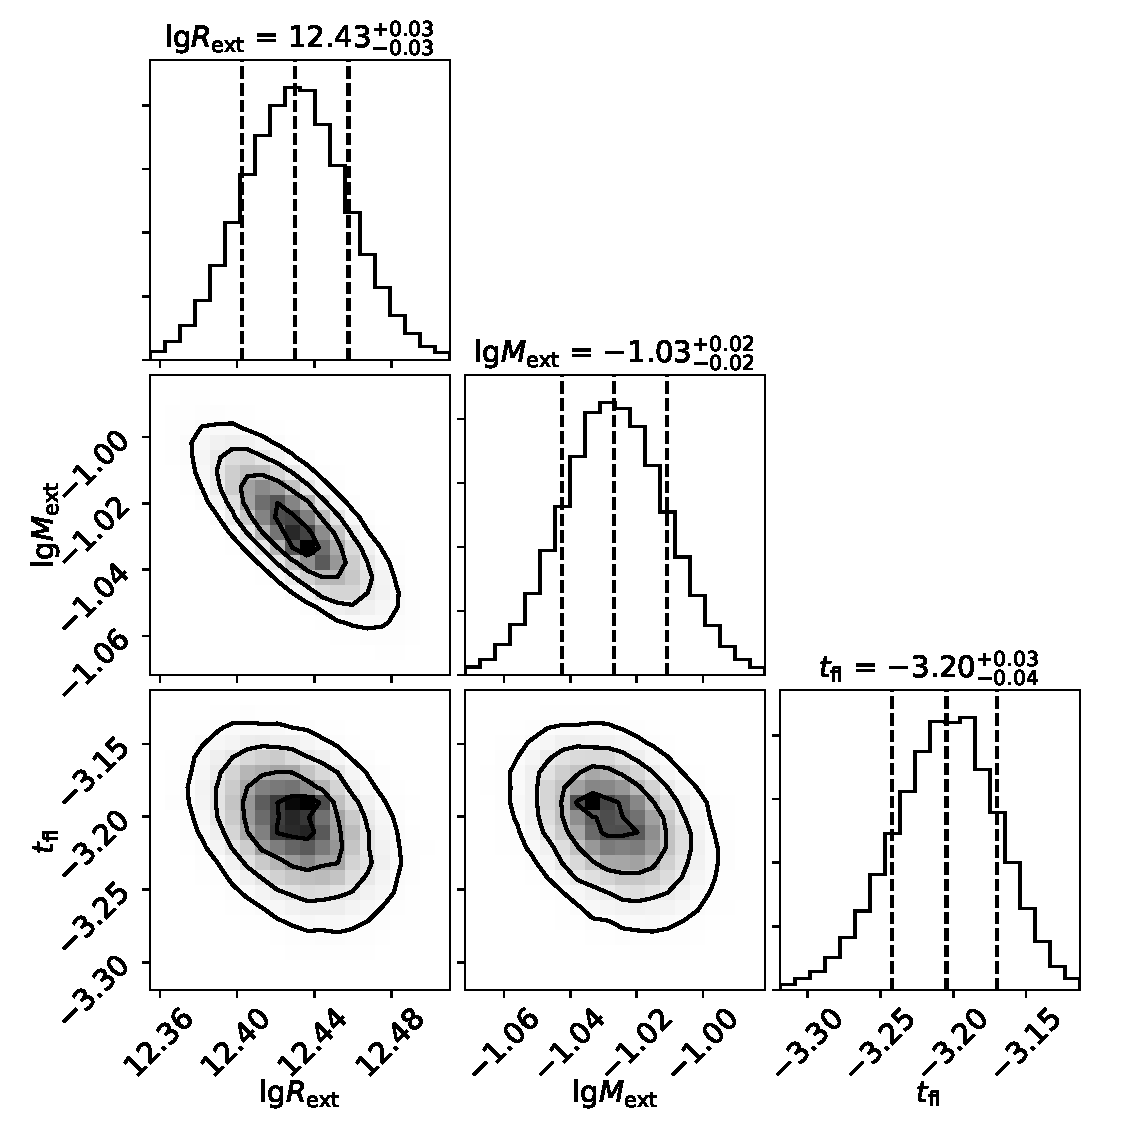
\includegraphics[width=\columnwidth]{figures/corner_P15.pdf}
	\caption{Corner plot showing the posterior constraints on ${\rm lg}R_{\rm ext}$, ${\rm lg}M_{\rm 
			ext}$, $t_\mathrm{fl}$, and $E_{\rm ext, 49}$. Marginalized one-dimensional distributions are 
			shown along the diagonal, along with the median estimate and the 68\% credible region (shown 
			with vertical 
		dashed 
		lines).	\label{fig:pirocorner}}
\end{figure}
We cast the P15 analytical expression for the shape of the early-time light curve in terms of $M_{\rm 
ext}$, $R_{\rm ext}$, $E_{\rm ext}$, and $E_{51}$:
\begin{subequations}
\begin{align}
 L(t) =& \frac{t_eE_{\rm ext}}{t_p^2} {\rm exp} \left[ -\frac{t (t + 2t_e)}{2t_p^2}\right] \,{\rm erg\, s^{-1}}\\
 t_e =& 10^{-9} R_{\rm ext} E_{\rm ext,49}^{-1/2} 
 \left(\frac{M_{\rm ext}}{0.01 M_\odot}\right)^{1/2} \, {\rm s}\\
 t_p =& 1.1\times 10^{5} \kappa_{34}^{1/2}  E_{51}^{-0.01 / 
 	1.4} \notag \\
 & \times E_{\rm ext, 49}^{-0.17 / 0.7}   \left(\frac{M_{\rm ext}}{0.01 M_\odot}\right)^{0.74} {\rm s} 
 \label{eq:tp}
\end{align}
\end{subequations}
where $t$ is time since explosion in seconds, $\kappa_{34} = \kappa / (0.34\,{\rm cm^2\, g^{-1}})$, 
$E_{\rm ext, 49} =  E_{\rm ext} / 
(10^{49}\,{\rm erg\,s^{-1}})$, $E_{51} =E /  (10^{51}\,{\rm 
erg\,s^{-1}})$, and $E$ is energy of the explosion.
Following P15 we assume the emission is a blackbody at radius
\begin{align*}
R(t) = R_{\rm ext} + 10^9  \left( \frac{E_{\rm ext}}{10^{49}\,{\rm 
		erg\,s^{-1}}} \right)^{1/2}  \left(\frac{M_{\rm ext}}{0.01 M_\odot}\right)^{-0.5} t
\end{align*}
and temperature
\begin{align*}
 T(t) = \left( \frac{L(t)}{4\pi R(t)^2 \sigma_{\rm SB}} \right)^{1/4}
\end{align*}

We fix $\kappa \approx 0.2\,{\rm cm^2\, g^{-1}}$ as 
appropriate for a hydrogen-deficient ionized gas, and assign wide flat priors for all model parameters, 
as summarized in Table~\ref{tab:P15priors}. We only include observations up to $\Delta t = 2$\,d in 
the fitting. We found that this particular choice of $\Delta t$ --- 2\,d instead of 1\,d or 3\,d --- in 
general does not affect the final inference for the model parameters. Figure~\ref{fig:pirocorner} shows 
the corner plot of ${\rm lg}R_{\rm ext}$, ${\rm lg}M_{\rm 	ext}$, $t_\mathrm{fl}$, and $E_{\rm ext, 49}$. 
For clarity, $E_{51}$ is excluded as it does not exhibit strong covariance with the parameters shown 
here. This can be understood by Eq.~\ref{eq:tp}, which gives $t_p \propto E_{51}^{-0.01/1.4}$, 
suggesting that the shock cooling luminosity only weakly depends on $E_{51}$. 

\begin{figure}[htbp!]
	\centering
	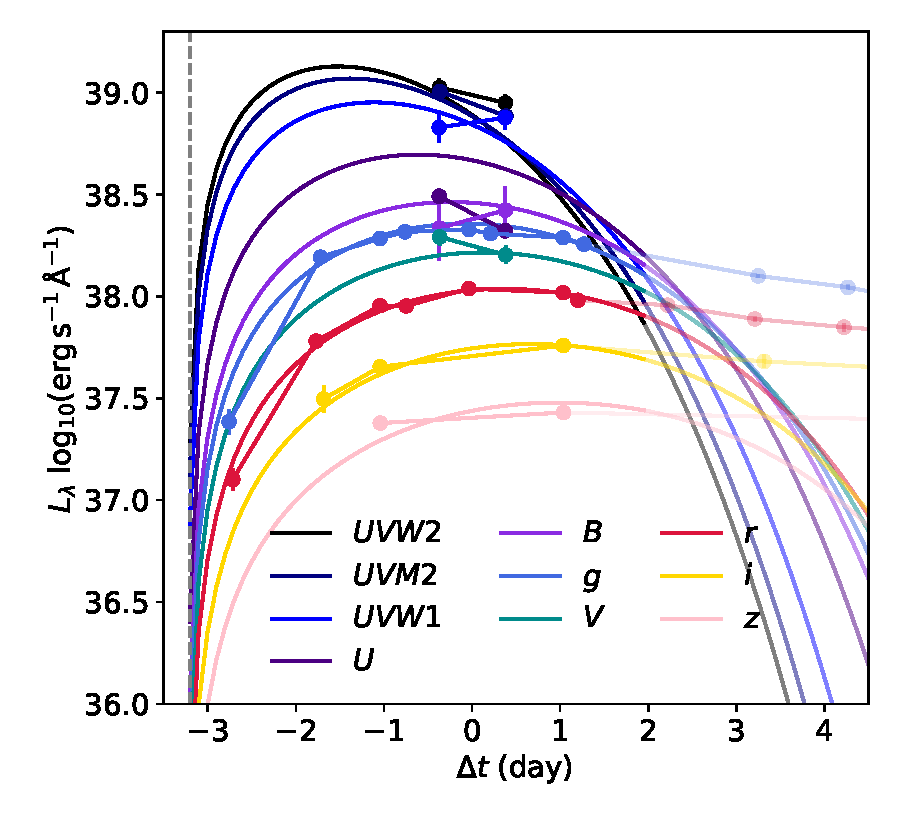
\includegraphics[width=\columnwidth]{figures/P15model.pdf}
	\caption{Cooling emission model fit to the early light curve of AT2019dge. 
		Data excluded from the fitting are shown as transparent circles. 
		The maximum a posteriori model is shown via solid lines.
		The vertical dashed line shows the median 1-D marginalized posterior value of
		$t_{\rm fl}$.
		\label{fig:piromodel}}
\end{figure}

The maximum a posteriori model is visualized by solid lines in Figure~\ref{fig:piromodel} color-coded in 
different filters. Note that the fitting is not perfect at the UV bands since 
the SED is not exactly a blackbody at peak (see Figure~\ref{fig:seds}). The rising part of the model 
does not closely match to data due to the ignorance of the density structure of the stellar profile. 
Nevertheless, the peak of the light curve is well captured by this model.

\subsection{Modelling the Main Peak}\label{subsec:arnettfit}

For $^{56}\rm Ni \rightarrow ^{56}Co \rightarrow ^{56}Fe$ decay powered explosions, the energy 
deposition rate is
\begin{align}
\varepsilon_{\rm rad} =&\varepsilon_{\rm Ni, \gamma} (t) + \varepsilon_{\rm Co, \gamma} (t) 
\label{eq:heatTotal} \\
\varepsilon_{\rm Ni, \gamma} (t)   =& \epsilon_{\rm Ni}e^{-t/\tau_{\rm Ni}}  \label{eq:heatNi}\\
\varepsilon_{\rm Co, \gamma} (t)   =& \epsilon_{\rm Co} \left( e^{-t/\tau_{\rm Co}} - e^{-t/\tau_{\rm 
			Ni}} \right) \label{eq:heatCo}
\end{align}
where $\epsilon_{\rm Ni}= 3.90 \times 10^{10} \, {\rm erg\,g^{-1}\,s^{-1}}$, $\epsilon_{\rm Co}=6.78\times 
10^{9} \, {\rm erg\,g^{-1}\,s^{-1}}$, $\tau_{\rm Ni}=8.8$\,d and $\tau_{\rm Co}=111.3$\,d are the decay 
lifetimes of $^{56}\rm Ni$ 
and $^{56}\rm Co$ \citep{Nadyozhin1994}. The effective heating rate is modified by the probability of 
thermalization, and thus $\varepsilon_{\rm heat} \leq \varepsilon_{\rm rad}$.

The bolometric light curve can be generally divided into the 
photospheric phase and the nebula phase. The photospheric phase can be modelled using Equations 
given in \citet[][Appendix A]{Valenti2008}, with modifications given 
by \citet[][Eq.~3]{Lyman2016}, 
\begin{align}
 L_{\rm phot} (t) =& M_{\rm Ni} {\rm e}^{-x^2} \times \notag  \\
 & \Big[ (\epsilon_{\rm Ni} - \epsilon_{\rm Co}) \int_0^x (2z {\rm e}^{-2zy+z^2}){\rm d} z \notag \\
 & + \epsilon_{\rm Co} \int_0^x (2z {\rm e}^{-2zy+2zs + z^2}) {\rm d} z \Big]
\end{align}
where $x = t/\tau_{\rm m}$, $y = \tau_{\rm m} / (2\tau_{\rm Ni})$,
\begin{align}
s &= \frac{\tau_{\rm m} (\tau_{\rm Co} - \tau_{\rm Ni})}{2 \tau_{\rm Co} \tau_{\rm Ni}}, \notag \\
\tau_{\rm m} &= \left( \frac{2\kappa_{\rm opt} M_{\rm ej}}{13.8 c v_{\rm phot}}\right)^{1/2}  
\label{eq:taum}
\end{align}

At the nebula phase the SN ejecta becomes optically thin, such that the delay between the energy 
deposition from radioactivity and the optical radiation becomes shorter. The bolometric luminosity is 
then equal to 
the rate of energy deposition: $L_{\rm neb}(t) = Q(t)$. At any given time, the energy deposition rate 
$Q(t)$ is \citep{Wheeler2015, Wygoda2019}:
\begin{align}
Q(t) \approx Q_{\gamma}(t) \left( 1 - e^{-(t_0/t)^2}\right) % Q_{\rm pos}(t),
\end{align}
where $Q_{\gamma}(t) = M_{\rm Ni}\varepsilon_{\rm rad}$ is the energy release rate of gamma-rays,
$t_0$ is the time at which the ejecta becomes optically thin to gamma rays. Here the difference 
between energy deposition rate of gamma-rays and positrons  is neglected.
%\begin{align}
%Q_{\rm pos}(t) &= M_{\rm Ni}\varepsilon_{\rm Co, pos}(t)\\
%\varepsilon_{\rm Co, pos}(t) &=  2.3\times 10^{8} \left( e^{-t/t_{s, {\rm Co}}} - e^{-t/t_{s, {\rm Ni}}}\right)
%\end{align}

\begin{deluxetable}{llc}[htpb!]
	\tablecaption{$^{56}$Ni decay model parameters $\theta$ and their priors \label{tab:Nidecaypriors}}
	\tablehead{
		\colhead{$\theta$}
		& \colhead{Description}
		&\colhead{Prior}
	}
	\startdata
	$\tau_{\rm m}$ &characteristic photon diffusion time in day  & $\mathcal{U}(1, 20)$ \\
	${\rm log}M_{\rm Ni}$ &  log$_{10}$ of nickel mass in $M_\odot$  & $\mathcal{U}(-4, 0)$\\
	$t_0$ & characteristic $\gamma$-ray escape time in day & $\mathcal{U}(20,  100)$  \\
	\enddata
\end{deluxetable}

\begin{figure}[htbp!]
	\centering
	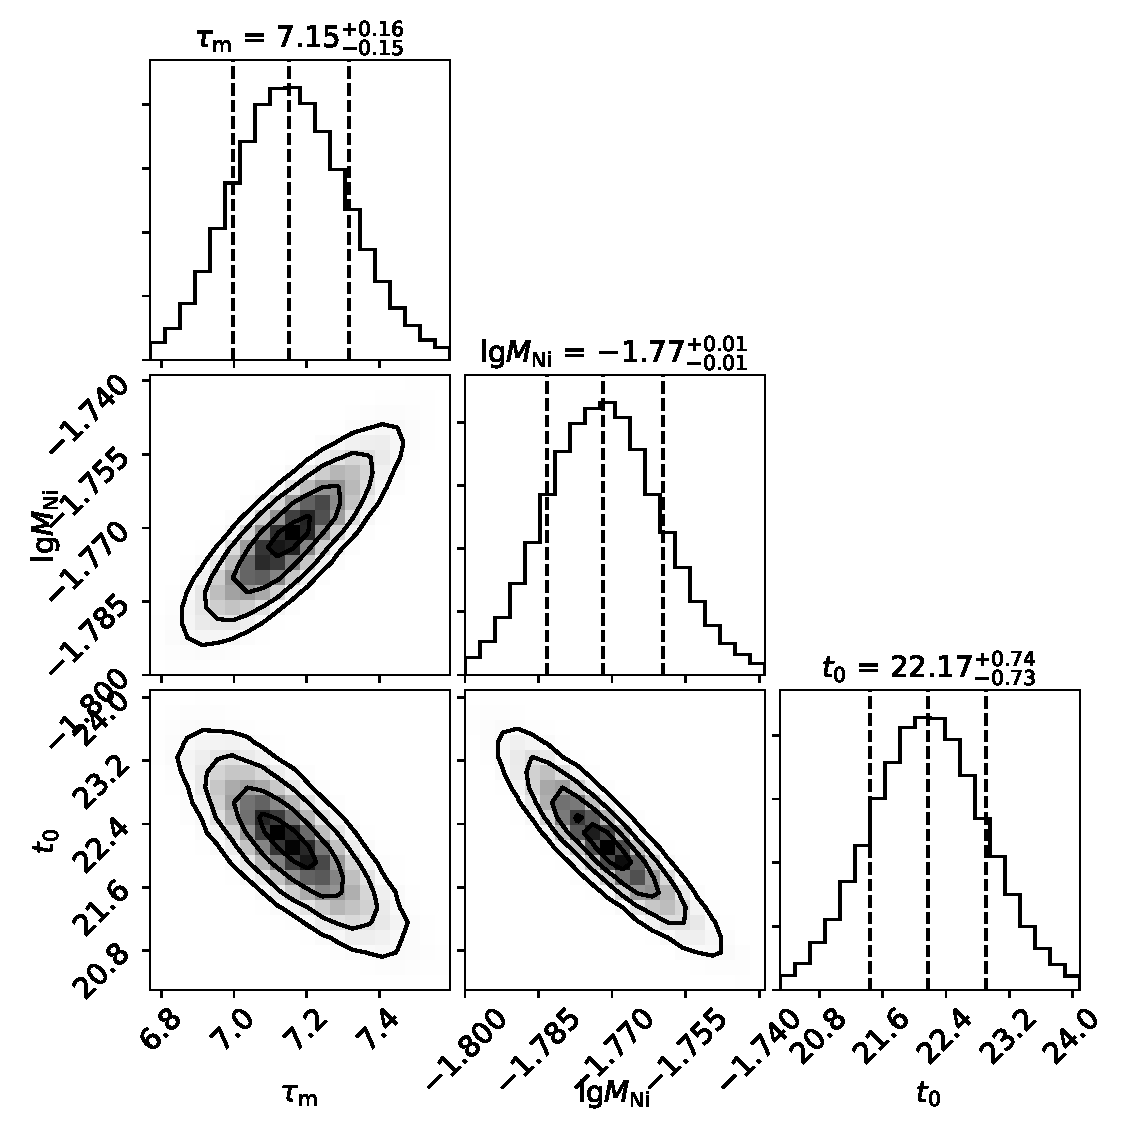
\includegraphics[width=\columnwidth]{figures/corner_arnett_modified.pdf}
	\caption{Corner plot showing the posterior constraints on $\tau_{\rm m}$, ${\rm lg}M_{\rm 
			Ni}$, and $t_0$. Marginalized one-dimensional distributions are shown along the 
		diagonal, along with the median estimate and the 68\% credible region (shown with vertical 
		dashed 
		lines).	\label{fig:Nidecaycorner}}
\end{figure}

To fit the shock cooling subtracted bolometric light curve with a simple radioactive decay model, we do 
not divide the data into photosperic phase and nebula phase, but instead adopt the following formula 
for the whole light curve:
\begin{align}
	L(t) = L_{\rm phot}(t)  \left( 1 - e^{-(t_0/t)^2}\right) 
\end{align}
Priors or the model parameters are summarized in Table~\ref{tab:Nidecaypriors}, and Figure 
\ref{fig:Nidecaycorner} shows the coner plot of $\tau_{\rm m}$, lg$M_{\rm Ni}$, and $t_0$.

\section{UV and Optical Spectroscopy} \label{sec:appspec}
\subsection{Data} \label{subsec:appspec_data}
The log of UV and optical spectroscopy is presented in Table \ref{tab:spec}.

\begin{table*}
	\caption{Log of AT2019dge spectroscopy. \label{tab:spec}}
	\centering
	\begin{tabular}{llrccc}
	\toprule
	Start Time  & Instrument & $\Delta t$& Exposure Time & Airmass & Resolution\\
	(UTC) & & (day)& & (s)& (FWHM $\AA$)\\
	\midrule
	% # DATE-OBS= '2019-04-09T03:30:28.157'             % # UTSTART = '03:30:28.157'
	% # MJD     =         58582.146159
	2019 Apr 09 03:30:28 & LT+SPART  & $-1.1$&  500   & 1.800 & 18 \\
	% # DATE-OBS= '2019-04-10T03:06:09.604'
	% # UTSTART = '03:06:09.604'
	% # MJD     =         58583.129278
	2019 Apr 10 03:06:10 & LT+SPART & $-0.1$ &  500   & 1.800 & 18 \\
	% LRIS
	2019 Apr 10 14:21:44 & Keck1+LRIS & $+0.4$ & 300 & 1.169 & 6 \\
	% HST
	2019 Apr 12 05:08:00 & HST+WFC3+UVIS & $+12.0$& 2$\times$250 & --- & 43\\
	% DBSP
	2019 Apr 24 11:06:43 & P200+DBSP & $+14.3$& 1200 & 1.047 & 3--5\\
	% LRIS
	2019 Jul 04 11:49:18   & Keck1+LRIS & $+85.3$& 1740 & 1.421 & 6\\
	% LRIS
	2019 Aug 31 08:04:58   & Keck1+LRIS &$+143.1$ & 1150 & 1.409 & 6  \\
	% LRIS
	2019 Sep 28 08:14:27   & Keck1+LRIS & $+171.1$& 600 & 2.165 & 6\\
	% LRIS
	2020 Feb 18 15:23:40   & Keck1+LRIS & $+314.4$& 1450 & 1.384 & 6\\
	\bottomrule
\end{tabular}
\end{table*}

%The final spectrum taken was a LRIS spectrum from $+111?$\,days which showed narrow nebular 
%emission lines from the host galaxy but no detectable flux from AT2019dge. 
We use line centers of nebular lines to derive the spectroscopic redshift of the host (Table 
\ref{tab:eml_host}). The mean of all centroids gives $z = 0.0213 \pm 0.0001$.

\begin{table}[htbp!]
	\caption{Line fluxes from the host galaxy of AT2019dge extracted from the Keck/LRIS spectrum 
	obtained on Aug xx 2019. }\label{tab:eml_host}
	\centering
	\begin{tabular}{llcc}
		\toprule
		Transition			& $\lambda_{\rm obs}$& $F$	\\
		& (\AA)	& $\left(10^{-16}~{\rm erg\,cm}^{-2}\,{\rm s}^{-1}\right) $ \\
		\midrule
		%{[\ion{O}{2}]}$\lambda\lambda$3726,3729 &$ 3848.17 \pm 0.05	$&$	334.5	\pm	6.23	$\\
		%{[\ion{Ne}{3}]}$\lambda$3869			& $ 3993.50 \pm 0.16	$&$	82.34	\pm	6.18	$\\
		%\ion{He}{1}$\lambda$3889,H-8			& $ 4014.49 \pm 0.16	$&$	29.01	\pm	4.73	$\\
		%{[\ion{Ne}{3}]}$\lambda$3968,H$\epsilon$& $ 4096.66 \pm 0.26	$&$	36.61	\pm	3.98	$\\
		%H$\delta$ 								& $ 4233.87 \pm 0.13	$&$	44.88	\pm	2.59	$\\
		%H$\gamma$								& $ 4480.20 \pm 0.10	$&$	81.95	\pm	3.74	$\\
		%{[\ion{O}{3}]}$\lambda$4364 			& $ 4503.68 \pm 0.10	$&$	15.01	\pm	2.69	$\\
		H$\beta$								& $ 4862.35 \pm 0.21	$ &$	32.45 \pm 2.08		$\\%yes
		%{[\ion{O}{3}]}$\lambda$4960 			& $ 5118.61 \pm 0.04	$&$	352.42	\pm	6.50	$\\
		{[\ion{O}{III}]}$\lambda$5007				& $5007.06 \pm 0.55$ &$67.56 \pm 13.52	$\\%yes
		%\ion{He}{1}$\lambda$5877				& $ 6064.21 \pm 0.20	$&$	27.04	\pm	2.30	$\\
		%\ion{O}{1}$\lambda$6302				& $ 6502.18 \pm 1.08	$&$	6.72	\pm	2.94	$\\
		%{[\ion{N}{2}]}$\lambda$6549				& $ 6758.16 \pm 0.02	$&$	11.15	\pm	6.73	$\\
		H$\alpha$								&$6562.07 	\pm 0.03$   & $115.79 \pm 1.16	$\\%yes
		{[\ion{N}{II}]}$\lambda$6583				& $6582.62 \pm 0.08$ &$	8.89 \pm 0.37	$\\%yes
		%{[\ion{He}{1}]}$\lambda$6678			& $ 6890.29 \pm 0.14	$&$	7.88	\pm	2.19	$\\
		%{[\ion{S}{2}]}$\lambda$6718 			& $ 6931.83 \pm 0.10	$&$	41.76	\pm	2.38	$\\
		%{[\ion{S}{2}]}$\lambda$6732 			& $ 6946.68 \pm 0.10	$&$	28.15	\pm	2.19	$\\
		\bottomrule
	\end{tabular}
	\tablecomments{All measurements are corrected for Galactic reddening.}
\end{table}
% no record in URAT1
% no record in GALEX



\bibliography{at2019dge}{}
\bibliographystyle{aasjournal}

\end{CJK*}


\end{document}